% =====================================================================
%  FangMath — Algebra 2, 6-7 Inverse Relations & Functions
%  One source file, two PDFs:
%    pdflatex -jobname=G7_Trig_First_Steps_Worksheet G7_Trig_First_Steps.tex
%    pdflatex -jobname=G7_Trig_First_Steps_Key "\def\iskey{1}% =====================================================================
%  FangMath — Algebra 2, 6-7 Inverse Relations & Functions
%  One source file, two PDFs:
%    pdflatex -jobname=G7_Trig_First_Steps_Worksheet G7_Trig_First_Steps.tex
%    pdflatex -jobname=G7_Trig_First_Steps_Key "\def\iskey{1}% =====================================================================
%  FangMath — Algebra 2, 6-7 Inverse Relations & Functions
%  One source file, two PDFs:
%    pdflatex -jobname=G7_Trig_First_Steps_Worksheet G7_Trig_First_Steps.tex
%    pdflatex -jobname=G7_Trig_First_Steps_Key "\def\iskey{1}% =====================================================================
%  FangMath — Algebra 2, 6-7 Inverse Relations & Functions
%  One source file, two PDFs:
%    pdflatex -jobname=G7_Trig_First_Steps_Worksheet G7_Trig_First_Steps.tex
%    pdflatex -jobname=G7_Trig_First_Steps_Key "\def\iskey{1}\input{G7_Trig_First_Steps.tex}"
% =====================================================================
\documentclass[12pt,letterpaper]{article}
\usepackage[margin=0.8in,top=0.85in,bottom=0.8in]{geometry}
\usepackage{mathpazo}
\usepackage[T1]{fontenc}
\usepackage{amsmath,amssymb}
\usepackage{xcolor}
\usepackage{enumitem}
\usepackage{multicol}
\usepackage{booktabs}
\usepackage{needspace}
\usepackage{fancyhdr}
\usepackage[most]{tcolorbox}
\usepackage{pgfplots}
\pgfplotsset{compat=1.17}
\usetikzlibrary{arrows.meta,calc}

\definecolor{FangBlue}{HTML}{1F4E79}
\definecolor{FangTeal}{HTML}{0F7C7C}
\definecolor{FangGold}{HTML}{C9962B}
\definecolor{FangRed}{HTML}{B3261E}
\definecolor{FangGreen}{HTML}{2E8B57}
\definecolor{FangPurple}{HTML}{6A4BD8}
\definecolor{Soft}{HTML}{F4F7FB}
% black-and-white version: pdflatex with \def\isbw{1} before \input
\ifdefined\isbw
\definecolor{FangBlue}{HTML}{000000}\definecolor{FangTeal}{HTML}{000000}\definecolor{FangGold}{HTML}{555555}
\definecolor{FangRed}{HTML}{000000}\definecolor{FangGreen}{HTML}{000000}\definecolor{FangPurple}{HTML}{000000}\definecolor{Soft}{HTML}{FFFFFF}
\fi

\newif\ifkey
\ifdefined\iskey \keytrue \else \keyfalse \fi

\pagestyle{fancy}\fancyhf{}
\renewcommand{\headrulewidth}{0.4pt}
\fancyhead[L]{\small\color{FangBlue}\textbf{FangMath} \,|\, Grade 7 \,·\, First Steps in Trigonometry}
\fancyhead[R]{\small\ifkey\textcolor{FangRed}{\textbf{ANSWER KEY}}\else Name: \underline{\hspace{4.2cm}}\fi}
\fancyfoot[C]{\small\thepage}
\fancyfoot[R]{\scriptsize\color{gray}fangmath.com}
\setlength{\headheight}{14pt}
\setlength{\parindent}{0pt}
\setlength{\parskip}{4pt}

% ---------- boxes ----------
\newtcolorbox{idea}[1][]{colback=Soft,colframe=FangBlue,boxrule=0.8pt,arc=3pt,left=8pt,right=8pt,top=6pt,bottom=6pt,
  fonttitle=\bfseries,coltitle=white,colbacktitle=FangBlue,title={#1}}
\newtcolorbox{example}[1][]{colback=white,colframe=FangTeal,boxrule=0.6pt,arc=3pt,left=8pt,right=8pt,top=5pt,bottom=5pt,
  fonttitle=\bfseries,coltitle=FangTeal,colbacktitle=white,title={#1},attach boxed title to top left={xshift=8pt,yshift=-7pt},boxed title style={boxrule=0pt,colframe=white}, enhanced}
\newtcolorbox{warn}{colback=FangRed!5,colframe=FangRed,boxrule=0.6pt,arc=3pt,left=8pt,right=8pt,top=4pt,bottom=4pt,leftrule=3pt}
\newtcolorbox{simple}{colback=FangGold!10,colframe=FangGold,boxrule=0.6pt,arc=3pt,left=8pt,right=8pt,top=4pt,bottom=4pt,leftrule=3pt}
\newtcolorbox{sol}{colback=FangGreen!6,colframe=FangGreen,boxrule=0.5pt,arc=2pt,left=6pt,right=6pt,top=3pt,bottom=3pt,breakable}

\newcommand{\badge}[2]{\tcbox[on line,colback=#1,colframe=#1,coltext=white,boxrule=0pt,arc=6pt,left=4pt,right=4pt,top=1pt,bottom=1pt,fontupper=\scriptsize\bfseries]{#2}}
\newcommand{\easy}{\badge{FangGreen}{EASY}}
\newcommand{\medium}{\badge{FangTeal}{MEDIUM}}
\newcommand{\hard}{\badge{FangRed}{HARD}}
\newcommand{\work}[2][]{\ifkey\begin{sol}#2\end{sol}\else\vspace*{#1}\fi}
\newcommand{\np}[1][6cm]{\needspace{#1}}
\newcommand{\sect}[2]{\par\needspace{7cm}\medskip{\Large\bfseries\color{FangBlue}\tcbox[on line,colback=FangBlue,colframe=FangBlue,coltext=white,arc=2pt,boxrule=0pt,left=5pt,right=5pt,top=1pt,bottom=1pt]{#1}\ #2}\par\smallskip}

% ---------- right-triangle picture: \rt{scale}{a}{b}{labels...} ----------
% vertices: C = right angle at origin, A = (b,0) [the angle we look from], B = (0,a)
\newcommand{\tri}[7][1]{% #2 #3 = legs (vertical, horizontal); #4 vertical label, #5 horizontal label, #6 hyp label, #7 angle label
\begin{tikzpicture}[scale=#1,font=\small]
\coordinate (C) at (0,0); \coordinate (A) at (#3,0); \coordinate (B) at (0,#2);
\draw[thick,FangBlue,fill=FangBlue!6] (C)--(A)--(B)--cycle;
\draw (0.28,0)--(0.28,0.28)--(0,0.28);
\node[left] at ($(C)!0.5!(B)$) {#4};
\node[below] at ($(C)!0.5!(A)$) {#5};
\node[above right] at ($(A)!0.5!(B)$) {#6};
\node[FangRed] at ($(A)+(-0.75,0.22)$) {#7};
\draw[FangRed,thick] ($(A)+(-0.5,0)$) arc[start angle=180,end angle={180-atan(#2/#3)},radius=0.5];
\end{tikzpicture}}

\begin{document}

% ======================= TITLE =======================
\begin{center}
{\color{FangBlue}\Huge\bfseries First Steps in Trigonometry}\\[3pt]
{\large Sine, Cosine and Tangent — the secret ratios inside every right triangle}
\ifkey\\[3pt]{\color{FangRed}\large\bfseries Answer Key}\fi
\end{center}
\vspace{-2pt}

\begin{idea}[The big idea]
\textbf{Trigonometry} (``triangle measuring'') lets you find a length you \emph{can't} measure — the height of a tree, a building, a kite — from one length and one angle you \emph{can} measure.\par
It works because in a right triangle, \textbf{the angle decides the shape}, and the shape decides the \textbf{ratios} of the sides.
\end{idea}

% ======================= PART 1 =======================
\sect{1}{Name the sides — always from the angle you are looking at}

\begin{minipage}[c]{0.44\textwidth}\centering
\tri[1.05]{3}{4}{\textbf{opposite}}{\textbf{adjacent}}{\textbf{hypotenuse}}{$A$}
\end{minipage}\hfill
\begin{minipage}[c]{0.54\textwidth}
Stand at the angle $A$ (the red arc) and look into the triangle:
\begin{itemize}[leftmargin=*,itemsep=3pt]
\item \textbf{Hypotenuse} — the longest side, \textbf{across from the right angle} $\llcorner$. It never changes.
\item \textbf{Opposite} — the side \textbf{across from} angle $A$. It doesn't touch $A$.
\item \textbf{Adjacent} — the side \textbf{next to} angle $A$ that is \emph{not} the hypotenuse. (``Adjacent'' means ``next to.'')
\end{itemize}
\end{minipage}

\begin{warn}
\textbf{Watch out:} opposite and adjacent \textbf{swap} if you stand at the other sharp angle. Always ask first: ``Which angle am I looking from?''
\end{warn}

% ======================= PART 2 =======================
\sect{2}{Why ratios? A simple case with three triangles}

\begin{minipage}[c]{0.5\textwidth}\centering
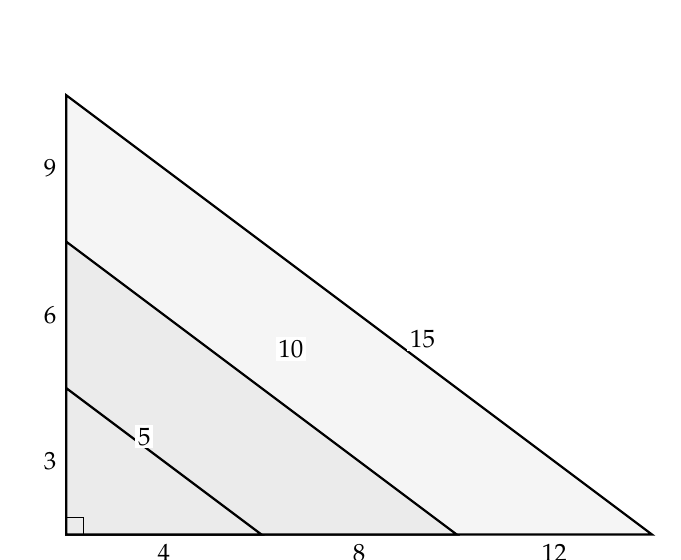
\begin{tikzpicture}[scale=0.62,font=\small]
\draw[thick,FangBlue,fill=FangBlue!4] (0,0)--(12,0)--(0,9)--cycle;
\draw[thick,FangTeal,fill=FangTeal!8] (0,0)--(8,0)--(0,6)--cycle;
\draw[thick,FangRed,fill=FangRed!8] (0,0)--(4,0)--(0,3)--cycle;
\draw (0.35,0)--(0.35,0.35)--(0,0.35);
\node[below,FangRed] at (2,0) {4}; \node[below,FangTeal] at (6,0) {8}; \node[below,FangBlue] at (10,0) {12};
\node[left,FangRed] at (0,1.5) {3}; \node[left,FangTeal] at (0,4.5) {6}; \node[left,FangBlue] at (0,7.5) {9};
\node[FangRed,fill=white,inner sep=1pt] at (1.6,2.0) {5}; \node[FangTeal,fill=white,inner sep=1pt] at (4.6,3.8) {10}; \node[FangBlue,fill=white,inner sep=1pt] at (7.3,4.0) {15};
\node at (-0.6,9.4) {};
\end{tikzpicture}
\end{minipage}\hfill
\begin{minipage}[c]{0.48\textwidth}
These are \textbf{scale drawings} of one triangle (scale factors $1$, $2$, $3$), so they all share the same angles. Look at $\dfrac{\text{opposite}}{\text{hypotenuse}}$ for the bottom-right angle:
\[\frac{3}{5}=0.6 \qquad \frac{6}{10}=0.6 \qquad \frac{9}{15}=0.6\]
\textbf{Same angle $\Rightarrow$ same ratio}, no matter how big the triangle is. These ratios get names: sine, cosine and tangent.
\end{minipage}

% ======================= PART 3 =======================
\sect{3}{The three definitions: SOH CAH TOA}

\begin{idea}[For an acute angle $A$ in a right triangle]
\[
\sin A=\frac{\textbf{O}\text{pposite}}{\textbf{H}\text{ypotenuse}}\qquad\quad
\cos A=\frac{\textbf{A}\text{djacent}}{\textbf{H}\text{ypotenuse}}\qquad\quad
\tan A=\frac{\textbf{O}\text{pposite}}{\textbf{A}\text{djacent}}
\]
\begin{center}\Large\bfseries\color{FangBlue} SOH \quad CAH \quad TOA\end{center}
\centering Memory sentence: \emph{\textbf{S}ome \textbf{O}ld \textbf{H}orses \textbf{C}an \textbf{A}lways \textbf{H}ear \textbf{T}heir \textbf{O}wners \textbf{A}pproach.}
\end{idea}

\begin{example}[Example 1 \;·\; read the ratios]
\begin{minipage}[c]{0.33\textwidth}\centering \tri[0.85]{3}{4}{$3$}{$4$}{$5$}{$A$}\end{minipage}\hfill
\begin{minipage}[c]{0.64\textwidth}
From angle $A$: opposite $=3$, adjacent $=4$, hypotenuse $=5$.
\[\sin A=\frac35=0.6\qquad \cos A=\frac45=0.8\qquad \tan A=\frac34=0.75\]
\textbf{Simple check:} sine and cosine are always \textbf{less than 1}, because the hypotenuse is the longest side.
\end{minipage}
\end{example}

% ======================= PART 4 =======================
\sect{4}{Use a table to find a missing side}

\begin{center}
\renewcommand{\arraystretch}{1.25}
\begin{tabular}{c|ccccc}
\toprule
\textbf{Angle} & $30^\circ$ & $37^\circ$ & $45^\circ$ & $53^\circ$ & $60^\circ$\\ \midrule
$\sin$ & $0.50$ & $0.60$ & $0.71$ & $0.80$ & $0.87$\\
$\cos$ & $0.87$ & $0.80$ & $0.71$ & $0.60$ & $0.50$\\
$\tan$ & $0.58$ & $0.75$ & $1.00$ & $1.33$ & $1.73$\\
\bottomrule
\end{tabular}\\[3pt]
{\small Values are rounded. (A scientific calculator gives them too — make sure it is in \textbf{degree} mode.)}
\end{center}

\begin{idea}[Four steps]
\textbf{1.} Mark the angle you know. \ \textbf{2.} Label the sides: hyp, opp, adj. \ \textbf{3.} Pick the ratio that uses the side you \emph{know} and the side you \emph{want}. \ \textbf{4.} Write the equation and solve it like a proportion.
\end{idea}

\begin{example}[Example 2 \;·\; how high does the ladder reach?]
\begin{minipage}[c]{0.33\textwidth}\centering \tri[0.65]{4.33}{2.5}{$h$\,?}{}{$10$ ft}{$60^\circ$}\end{minipage}\hfill
\begin{minipage}[c]{0.64\textwidth}
A $10$-foot ladder leans on a wall at a $60^\circ$ angle with the ground. \\
Know: hypotenuse $=10$. \ Want: the height, which is \textbf{opposite} the $60^\circ$ angle. \\
Opposite and hypotenuse $\Rightarrow$ \textbf{SOH}, sine:
\[\sin 60^\circ=\frac{h}{10}\ \Rightarrow\ 0.87=\frac{h}{10}\ \Rightarrow\ h=10\times0.87=8.7\ \text{ft}.\]
\end{minipage}
\end{example}

\begin{example}[Example 3 \;·\; the unknown is on the bottom]
The opposite side of a $30^\circ$ angle is $6$. How long is the hypotenuse? \quad
$\sin30^\circ=\dfrac{6}{h}\Rightarrow 0.5=\dfrac{6}{h}\Rightarrow h=\dfrac{6}{0.5}=12.$ \quad \textbf{Check:} $\frac{6}{12}=0.5$ \checkmark
\end{example}

% ======================= PRACTICE =======================
\sect{5}{Practice}

\needspace{6cm}{\large\bfseries\color{FangBlue}A.\ Name the sides} \easy

\textit{For the marked angle, write which side is the hypotenuse, the opposite and the adjacent.}

\begin{center}
\begin{tabular}{ccc}
\textbf{1.} \tri[0.7]{3}{4}{$p$}{$q$}{$r$}{$A$} &
\textbf{2.} 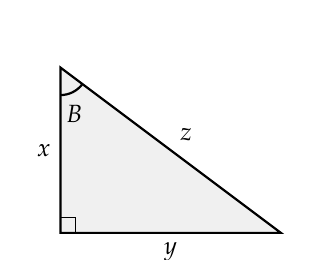
\begin{tikzpicture}[scale=0.7,font=\small]
\draw[thick,FangBlue,fill=FangBlue!6] (0,0)--(4,0)--(0,3)--cycle; \draw (0.28,0)--(0.28,0.28)--(0,0.28);
\node[left] at (0,1.5) {$x$}; \node[below] at (2,0) {$y$}; \node[above right] at (2,1.5) {$z$};
\node[FangRed] at (0.25,2.15) {$B$}; \draw[FangRed,thick] (0,2.5) arc[start angle=270,end angle={270+53.13},radius=0.5];
\end{tikzpicture} &
\textbf{3.} 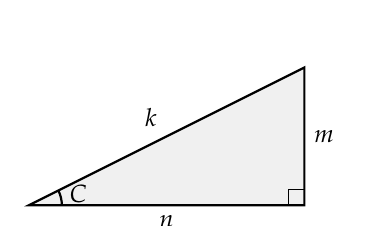
\begin{tikzpicture}[scale=0.7,font=\small]
\draw[thick,FangBlue,fill=FangBlue!6] (0,0)--(5,0)--(5,2.5)--cycle; \draw (4.72,0)--(4.72,0.28)--(5,0.28);
\node[right] at (5,1.25) {$m$}; \node[below] at (2.5,0) {$n$}; \node[above left] at (2.5,1.25) {$k$};
\node[FangRed] at (0.9,0.2) {$C$}; \draw[FangRed,thick] (0.6,0) arc[start angle=0,end angle=26.57,radius=0.6];
\end{tikzpicture}\\[2pt]
\ifkey{\small\color{FangGreen} hyp $r$, opp $p$, adj $q$}\else{\small hyp \underline{\hspace{0.7cm}} opp \underline{\hspace{0.7cm}} adj \underline{\hspace{0.7cm}}}\fi &
\ifkey{\small\color{FangGreen} hyp $z$, opp $y$, adj $x$}\else{\small hyp \underline{\hspace{0.7cm}} opp \underline{\hspace{0.7cm}} adj \underline{\hspace{0.7cm}}}\fi &
\ifkey{\small\color{FangGreen} hyp $k$, opp $m$, adj $n$}\else{\small hyp \underline{\hspace{0.7cm}} opp \underline{\hspace{0.7cm}} adj \underline{\hspace{0.7cm}}}\fi
\end{tabular}
\end{center}

\needspace{7cm}{\large\bfseries\color{FangBlue}B.\ Write the ratios} \easy\ \medium

\textit{Write $\sin A$, $\cos A$ and $\tan A$ as fractions in lowest terms, then as decimals (round to the hundredths).}

\begin{enumerate}[leftmargin=*,label=\textbf{\arabic*.},itemsep=6pt]
\setcounter{enumi}{3}
\np[4.5cm]\item \begin{minipage}[t]{0.3\textwidth}\vspace{0pt}\tri[0.55]{5}{12}{$5$}{$12$}{$13$}{$A$}\end{minipage}\hfill\begin{minipage}[t]{0.62\textwidth}\vspace{0pt}
\work[2.2cm]{opp $5$, adj $12$, hyp $13$. \ $\sin A=\frac{5}{13}\approx0.38$, \ $\cos A=\frac{12}{13}\approx0.92$, \ $\tan A=\frac{5}{12}\approx0.42$.}\end{minipage}
\np[4.5cm]\item \begin{minipage}[t]{0.3\textwidth}\vspace{0pt}\tri[0.32]{15}{8}{$15$}{$8$}{$17$}{$A$}\end{minipage}\hfill\begin{minipage}[t]{0.62\textwidth}\vspace{0pt}
\work[2.2cm]{opp $15$, adj $8$, hyp $17$. \ $\sin A=\frac{15}{17}\approx0.88$, \ $\cos A=\frac{8}{17}\approx0.47$, \ $\tan A=\frac{15}{8}=1.875\approx1.88$. \\ (A tangent \emph{can} be bigger than 1 — when the opposite side is longer than the adjacent.)}\end{minipage}
\np[4.5cm]\item \begin{minipage}[t]{0.3\textwidth}\vspace{0pt}\tri[0.5]{6}{8}{$6$}{$8$}{$10$}{$A$}\end{minipage}\hfill\begin{minipage}[t]{0.62\textwidth}\vspace{0pt}
\work[2.2cm]{$\sin A=\frac{6}{10}=\frac35=0.6$, \ $\cos A=\frac{8}{10}=\frac45=0.8$, \ $\tan A=\frac68=\frac34=0.75$. \\ Same as the $3$-$4$-$5$ triangle — it is a scale drawing (factor $2$), so it has the same angles.}\end{minipage}
\np[3.2cm]\item \medium\ In the triangle of problem 4, now stand at the \textbf{other} sharp angle $B$. Write $\sin B$, $\cos B$ and $\tan B$. What do you notice?
\work[2.2cm]{From $B$: opp $12$, adj $5$, hyp $13$. \ $\sin B=\frac{12}{13}$, \ $\cos B=\frac{5}{13}$, \ $\tan B=\frac{12}{5}$. \\ $\sin B=\cos A$ and $\cos B=\sin A$ — opposite and adjacent swapped. $\tan B$ is the reciprocal of $\tan A$.}
\end{enumerate}

\needspace{6cm}{\large\bfseries\color{FangBlue}C.\ Same angle, same ratio} \medium

\begin{enumerate}[resume,leftmargin=*,label=\textbf{\arabic*.},itemsep=6pt]
\np\item Triangle $P$ has legs $5$ and $12$. Triangle $Q$ has legs $10$ and $24$. Find $\tan$ of the angle across from the short leg in each. Are the two angles equal? Explain.
\work[2.4cm]{$P$: $\tan=\frac{5}{12}$. \ $Q$: $\tan=\frac{10}{24}=\frac{5}{12}$. \ Same ratio, so the angles are equal. $Q$ is a scale drawing of $P$ with scale factor $2$ — scaling changes lengths, not angles.}
\end{enumerate}

\needspace{6cm}{\large\bfseries\color{FangBlue}D.\ Which ratio?} \medium

\textit{Write sin, cos or tan. (Which two sides does the problem use?)}

\begin{enumerate}[resume,leftmargin=*,label=\textbf{\arabic*.},itemsep=4pt]
\item Know the hypotenuse, want the opposite. \work[0.4cm]{sin (SOH)}
\item Know the adjacent, want the opposite. \work[0.4cm]{tan (TOA)}
\item Know the hypotenuse, want the adjacent. \work[0.4cm]{cos (CAH)}
\item Know the opposite, want the hypotenuse. \work[0.4cm]{sin (SOH)}
\end{enumerate}

\needspace{6cm}{\large\bfseries\color{FangBlue}E.\ Find the missing side} \medium\ \hard

\textit{Use the table in Part 4. Draw a picture, label hyp / opp / adj, then solve.}

\begin{enumerate}[resume,leftmargin=*,label=\textbf{\arabic*.},itemsep=6pt]
\np\item \medium\ The hypotenuse is $20$ and one angle is $30^\circ$. Find the side opposite the $30^\circ$ angle.
\work[2.2cm]{$\sin30^\circ=\frac{x}{20}$, \ $0.5=\frac{x}{20}$, \ $x=20\times0.5=10$.}
\np\item \medium\ A ramp is $10$ m long and rises at an angle of $30^\circ$. How high does it go?
\work[2.2cm]{The ramp is the hypotenuse; the height is opposite: $\sin30^\circ=\frac{h}{10}$, \ $h=10\times0.5=5$ m.}
\np\item \medium\ One leg is $8$ and the angle next to it is $45^\circ$. Find the other leg (opposite the $45^\circ$ angle).
\work[2.2cm]{Adjacent $8$, want opposite: $\tan45^\circ=\frac{x}{8}$, \ $1=\frac{x}{8}$, \ $x=8$. \ (A $45^\circ$ right triangle has two equal legs.)}
\np\item \medium\ The hypotenuse is $15$ and one angle is $37^\circ$. Find the side adjacent to the $37^\circ$ angle.
\work[2.2cm]{$\cos37^\circ=\frac{x}{15}$, \ $0.8=\frac{x}{15}$, \ $x=15\times0.8=12$. \ (A $9$-$12$-$15$ triangle — a scaled $3$-$4$-$5$!)}
\np\item \medium\ A tree casts a shadow $12$ m long. From the tip of the shadow, the top of the tree is at an angle of $53^\circ$. How tall is the tree?
\work[2.4cm]{The shadow is adjacent to the $53^\circ$ angle; the tree is opposite. \ $\tan53^\circ=\frac{h}{12}$, \ $h=12\times1.33\approx16$ m.}
\np\item \hard\ The side opposite a $30^\circ$ angle is $7$. Find the hypotenuse.
\work[2.2cm]{$\sin30^\circ=\frac{7}{h}$, \ $0.5=\frac{7}{h}$, \ $h=\frac{7}{0.5}=14$. \ Check: $\frac{7}{14}=0.5$ \checkmark}
\np\item \hard\ A kite string is $50$ m long and makes a $37^\circ$ angle with the ground. How high is the kite? How far away along the ground is it?
\work[2.6cm]{Height (opposite): $50\times\sin37^\circ=50\times0.6=30$ m. \ Ground distance (adjacent): $50\times\cos37^\circ=50\times0.8=40$ m. \ ($30$-$40$-$50$: a scaled $3$-$4$-$5$ triangle.)}
\end{enumerate}

\needspace{6cm}{\large\bfseries\color{FangBlue}F.\ Think about it} \hard

\begin{enumerate}[resume,leftmargin=*,label=\textbf{\arabic*.},itemsep=6pt]
\np\item Why can $\sin A$ never be bigger than $1$?
\work[2cm]{$\sin A=\frac{\text{opposite}}{\text{hypotenuse}}$ and the hypotenuse is the longest side, so the top is smaller than the bottom: the fraction is less than $1$.}
\np\item In a right triangle, $\sin A=\frac35$ and the hypotenuse is $25$. Find the opposite side. Then use $\cos A=\frac45$ to find the adjacent side.
\work[2.2cm]{Opposite $=\frac35\times25=15$. \ Adjacent $=\frac45\times25=20$. \ ($15$-$20$-$25$ is the $3$-$4$-$5$ triangle scaled by $5$.)}
\np\item Why is $\tan45^\circ$ exactly $1$?
\work[2cm]{The angles are $90^\circ$, $45^\circ$, $45^\circ$, so two angles are equal and the two legs are equal. $\tan45^\circ=\frac{\text{opp}}{\text{adj}}=\frac{\text{same}}{\text{same}}=1$.}
\end{enumerate}

\ifkey\else
\vfill
\begin{simple}
\textbf{Remember:} 1) Mark the angle. \ 2) Label hyp, opp, adj from that angle. \ 3) SOH CAH TOA. \ 4) Check: does the hypotenuse come out the longest?
\end{simple}
\fi

\end{document}
"
% =====================================================================
\documentclass[12pt,letterpaper]{article}
\usepackage[margin=0.8in,top=0.85in,bottom=0.8in]{geometry}
\usepackage{mathpazo}
\usepackage[T1]{fontenc}
\usepackage{amsmath,amssymb}
\usepackage{xcolor}
\usepackage{enumitem}
\usepackage{multicol}
\usepackage{booktabs}
\usepackage{needspace}
\usepackage{fancyhdr}
\usepackage[most]{tcolorbox}
\usepackage{pgfplots}
\pgfplotsset{compat=1.17}
\usetikzlibrary{arrows.meta,calc}

\definecolor{FangBlue}{HTML}{1F4E79}
\definecolor{FangTeal}{HTML}{0F7C7C}
\definecolor{FangGold}{HTML}{C9962B}
\definecolor{FangRed}{HTML}{B3261E}
\definecolor{FangGreen}{HTML}{2E8B57}
\definecolor{FangPurple}{HTML}{6A4BD8}
\definecolor{Soft}{HTML}{F4F7FB}
% black-and-white version: pdflatex with \def\isbw{1} before \input
\ifdefined\isbw
\definecolor{FangBlue}{HTML}{000000}\definecolor{FangTeal}{HTML}{000000}\definecolor{FangGold}{HTML}{555555}
\definecolor{FangRed}{HTML}{000000}\definecolor{FangGreen}{HTML}{000000}\definecolor{FangPurple}{HTML}{000000}\definecolor{Soft}{HTML}{FFFFFF}
\fi

\newif\ifkey
\ifdefined\iskey \keytrue \else \keyfalse \fi

\pagestyle{fancy}\fancyhf{}
\renewcommand{\headrulewidth}{0.4pt}
\fancyhead[L]{\small\color{FangBlue}\textbf{FangMath} \,|\, Grade 7 \,·\, First Steps in Trigonometry}
\fancyhead[R]{\small\ifkey\textcolor{FangRed}{\textbf{ANSWER KEY}}\else Name: \underline{\hspace{4.2cm}}\fi}
\fancyfoot[C]{\small\thepage}
\fancyfoot[R]{\scriptsize\color{gray}fangmath.com}
\setlength{\headheight}{14pt}
\setlength{\parindent}{0pt}
\setlength{\parskip}{4pt}

% ---------- boxes ----------
\newtcolorbox{idea}[1][]{colback=Soft,colframe=FangBlue,boxrule=0.8pt,arc=3pt,left=8pt,right=8pt,top=6pt,bottom=6pt,
  fonttitle=\bfseries,coltitle=white,colbacktitle=FangBlue,title={#1}}
\newtcolorbox{example}[1][]{colback=white,colframe=FangTeal,boxrule=0.6pt,arc=3pt,left=8pt,right=8pt,top=5pt,bottom=5pt,
  fonttitle=\bfseries,coltitle=FangTeal,colbacktitle=white,title={#1},attach boxed title to top left={xshift=8pt,yshift=-7pt},boxed title style={boxrule=0pt,colframe=white}, enhanced}
\newtcolorbox{warn}{colback=FangRed!5,colframe=FangRed,boxrule=0.6pt,arc=3pt,left=8pt,right=8pt,top=4pt,bottom=4pt,leftrule=3pt}
\newtcolorbox{simple}{colback=FangGold!10,colframe=FangGold,boxrule=0.6pt,arc=3pt,left=8pt,right=8pt,top=4pt,bottom=4pt,leftrule=3pt}
\newtcolorbox{sol}{colback=FangGreen!6,colframe=FangGreen,boxrule=0.5pt,arc=2pt,left=6pt,right=6pt,top=3pt,bottom=3pt,breakable}

\newcommand{\badge}[2]{\tcbox[on line,colback=#1,colframe=#1,coltext=white,boxrule=0pt,arc=6pt,left=4pt,right=4pt,top=1pt,bottom=1pt,fontupper=\scriptsize\bfseries]{#2}}
\newcommand{\easy}{\badge{FangGreen}{EASY}}
\newcommand{\medium}{\badge{FangTeal}{MEDIUM}}
\newcommand{\hard}{\badge{FangRed}{HARD}}
\newcommand{\work}[2][]{\ifkey\begin{sol}#2\end{sol}\else\vspace*{#1}\fi}
\newcommand{\np}[1][6cm]{\needspace{#1}}
\newcommand{\sect}[2]{\par\needspace{7cm}\medskip{\Large\bfseries\color{FangBlue}\tcbox[on line,colback=FangBlue,colframe=FangBlue,coltext=white,arc=2pt,boxrule=0pt,left=5pt,right=5pt,top=1pt,bottom=1pt]{#1}\ #2}\par\smallskip}

% ---------- right-triangle picture: \rt{scale}{a}{b}{labels...} ----------
% vertices: C = right angle at origin, A = (b,0) [the angle we look from], B = (0,a)
\newcommand{\tri}[7][1]{% #2 #3 = legs (vertical, horizontal); #4 vertical label, #5 horizontal label, #6 hyp label, #7 angle label
\begin{tikzpicture}[scale=#1,font=\small]
\coordinate (C) at (0,0); \coordinate (A) at (#3,0); \coordinate (B) at (0,#2);
\draw[thick,FangBlue,fill=FangBlue!6] (C)--(A)--(B)--cycle;
\draw (0.28,0)--(0.28,0.28)--(0,0.28);
\node[left] at ($(C)!0.5!(B)$) {#4};
\node[below] at ($(C)!0.5!(A)$) {#5};
\node[above right] at ($(A)!0.5!(B)$) {#6};
\node[FangRed] at ($(A)+(-0.75,0.22)$) {#7};
\draw[FangRed,thick] ($(A)+(-0.5,0)$) arc[start angle=180,end angle={180-atan(#2/#3)},radius=0.5];
\end{tikzpicture}}

\begin{document}

% ======================= TITLE =======================
\begin{center}
{\color{FangBlue}\Huge\bfseries First Steps in Trigonometry}\\[3pt]
{\large Sine, Cosine and Tangent — the secret ratios inside every right triangle}
\ifkey\\[3pt]{\color{FangRed}\large\bfseries Answer Key}\fi
\end{center}
\vspace{-2pt}

\begin{idea}[The big idea]
\textbf{Trigonometry} (``triangle measuring'') lets you find a length you \emph{can't} measure — the height of a tree, a building, a kite — from one length and one angle you \emph{can} measure.\par
It works because in a right triangle, \textbf{the angle decides the shape}, and the shape decides the \textbf{ratios} of the sides.
\end{idea}

% ======================= PART 1 =======================
\sect{1}{Name the sides — always from the angle you are looking at}

\begin{minipage}[c]{0.44\textwidth}\centering
\tri[1.05]{3}{4}{\textbf{opposite}}{\textbf{adjacent}}{\textbf{hypotenuse}}{$A$}
\end{minipage}\hfill
\begin{minipage}[c]{0.54\textwidth}
Stand at the angle $A$ (the red arc) and look into the triangle:
\begin{itemize}[leftmargin=*,itemsep=3pt]
\item \textbf{Hypotenuse} — the longest side, \textbf{across from the right angle} $\llcorner$. It never changes.
\item \textbf{Opposite} — the side \textbf{across from} angle $A$. It doesn't touch $A$.
\item \textbf{Adjacent} — the side \textbf{next to} angle $A$ that is \emph{not} the hypotenuse. (``Adjacent'' means ``next to.'')
\end{itemize}
\end{minipage}

\begin{warn}
\textbf{Watch out:} opposite and adjacent \textbf{swap} if you stand at the other sharp angle. Always ask first: ``Which angle am I looking from?''
\end{warn}

% ======================= PART 2 =======================
\sect{2}{Why ratios? A simple case with three triangles}

\begin{minipage}[c]{0.5\textwidth}\centering
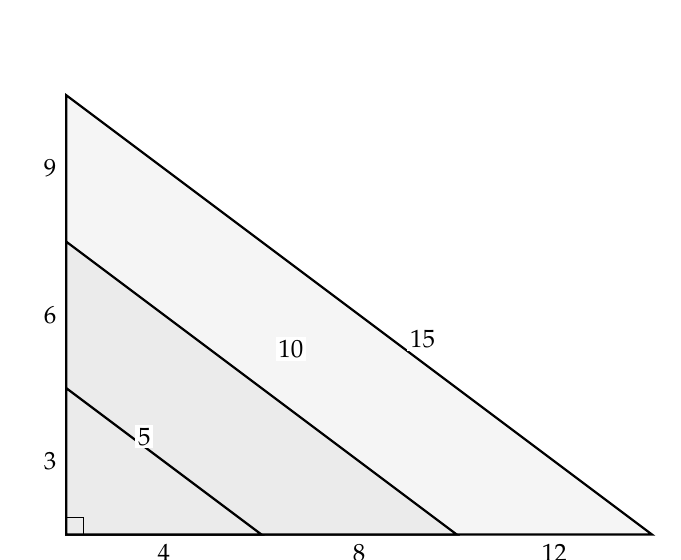
\begin{tikzpicture}[scale=0.62,font=\small]
\draw[thick,FangBlue,fill=FangBlue!4] (0,0)--(12,0)--(0,9)--cycle;
\draw[thick,FangTeal,fill=FangTeal!8] (0,0)--(8,0)--(0,6)--cycle;
\draw[thick,FangRed,fill=FangRed!8] (0,0)--(4,0)--(0,3)--cycle;
\draw (0.35,0)--(0.35,0.35)--(0,0.35);
\node[below,FangRed] at (2,0) {4}; \node[below,FangTeal] at (6,0) {8}; \node[below,FangBlue] at (10,0) {12};
\node[left,FangRed] at (0,1.5) {3}; \node[left,FangTeal] at (0,4.5) {6}; \node[left,FangBlue] at (0,7.5) {9};
\node[FangRed,fill=white,inner sep=1pt] at (1.6,2.0) {5}; \node[FangTeal,fill=white,inner sep=1pt] at (4.6,3.8) {10}; \node[FangBlue,fill=white,inner sep=1pt] at (7.3,4.0) {15};
\node at (-0.6,9.4) {};
\end{tikzpicture}
\end{minipage}\hfill
\begin{minipage}[c]{0.48\textwidth}
These are \textbf{scale drawings} of one triangle (scale factors $1$, $2$, $3$), so they all share the same angles. Look at $\dfrac{\text{opposite}}{\text{hypotenuse}}$ for the bottom-right angle:
\[\frac{3}{5}=0.6 \qquad \frac{6}{10}=0.6 \qquad \frac{9}{15}=0.6\]
\textbf{Same angle $\Rightarrow$ same ratio}, no matter how big the triangle is. These ratios get names: sine, cosine and tangent.
\end{minipage}

% ======================= PART 3 =======================
\sect{3}{The three definitions: SOH CAH TOA}

\begin{idea}[For an acute angle $A$ in a right triangle]
\[
\sin A=\frac{\textbf{O}\text{pposite}}{\textbf{H}\text{ypotenuse}}\qquad\quad
\cos A=\frac{\textbf{A}\text{djacent}}{\textbf{H}\text{ypotenuse}}\qquad\quad
\tan A=\frac{\textbf{O}\text{pposite}}{\textbf{A}\text{djacent}}
\]
\begin{center}\Large\bfseries\color{FangBlue} SOH \quad CAH \quad TOA\end{center}
\centering Memory sentence: \emph{\textbf{S}ome \textbf{O}ld \textbf{H}orses \textbf{C}an \textbf{A}lways \textbf{H}ear \textbf{T}heir \textbf{O}wners \textbf{A}pproach.}
\end{idea}

\begin{example}[Example 1 \;·\; read the ratios]
\begin{minipage}[c]{0.33\textwidth}\centering \tri[0.85]{3}{4}{$3$}{$4$}{$5$}{$A$}\end{minipage}\hfill
\begin{minipage}[c]{0.64\textwidth}
From angle $A$: opposite $=3$, adjacent $=4$, hypotenuse $=5$.
\[\sin A=\frac35=0.6\qquad \cos A=\frac45=0.8\qquad \tan A=\frac34=0.75\]
\textbf{Simple check:} sine and cosine are always \textbf{less than 1}, because the hypotenuse is the longest side.
\end{minipage}
\end{example}

% ======================= PART 4 =======================
\sect{4}{Use a table to find a missing side}

\begin{center}
\renewcommand{\arraystretch}{1.25}
\begin{tabular}{c|ccccc}
\toprule
\textbf{Angle} & $30^\circ$ & $37^\circ$ & $45^\circ$ & $53^\circ$ & $60^\circ$\\ \midrule
$\sin$ & $0.50$ & $0.60$ & $0.71$ & $0.80$ & $0.87$\\
$\cos$ & $0.87$ & $0.80$ & $0.71$ & $0.60$ & $0.50$\\
$\tan$ & $0.58$ & $0.75$ & $1.00$ & $1.33$ & $1.73$\\
\bottomrule
\end{tabular}\\[3pt]
{\small Values are rounded. (A scientific calculator gives them too — make sure it is in \textbf{degree} mode.)}
\end{center}

\begin{idea}[Four steps]
\textbf{1.} Mark the angle you know. \ \textbf{2.} Label the sides: hyp, opp, adj. \ \textbf{3.} Pick the ratio that uses the side you \emph{know} and the side you \emph{want}. \ \textbf{4.} Write the equation and solve it like a proportion.
\end{idea}

\begin{example}[Example 2 \;·\; how high does the ladder reach?]
\begin{minipage}[c]{0.33\textwidth}\centering \tri[0.65]{4.33}{2.5}{$h$\,?}{}{$10$ ft}{$60^\circ$}\end{minipage}\hfill
\begin{minipage}[c]{0.64\textwidth}
A $10$-foot ladder leans on a wall at a $60^\circ$ angle with the ground. \\
Know: hypotenuse $=10$. \ Want: the height, which is \textbf{opposite} the $60^\circ$ angle. \\
Opposite and hypotenuse $\Rightarrow$ \textbf{SOH}, sine:
\[\sin 60^\circ=\frac{h}{10}\ \Rightarrow\ 0.87=\frac{h}{10}\ \Rightarrow\ h=10\times0.87=8.7\ \text{ft}.\]
\end{minipage}
\end{example}

\begin{example}[Example 3 \;·\; the unknown is on the bottom]
The opposite side of a $30^\circ$ angle is $6$. How long is the hypotenuse? \quad
$\sin30^\circ=\dfrac{6}{h}\Rightarrow 0.5=\dfrac{6}{h}\Rightarrow h=\dfrac{6}{0.5}=12.$ \quad \textbf{Check:} $\frac{6}{12}=0.5$ \checkmark
\end{example}

% ======================= PRACTICE =======================
\sect{5}{Practice}

\needspace{6cm}{\large\bfseries\color{FangBlue}A.\ Name the sides} \easy

\textit{For the marked angle, write which side is the hypotenuse, the opposite and the adjacent.}

\begin{center}
\begin{tabular}{ccc}
\textbf{1.} \tri[0.7]{3}{4}{$p$}{$q$}{$r$}{$A$} &
\textbf{2.} 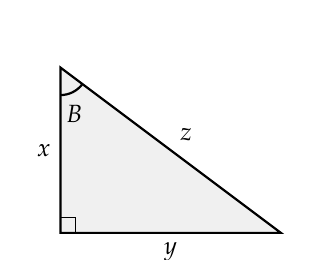
\begin{tikzpicture}[scale=0.7,font=\small]
\draw[thick,FangBlue,fill=FangBlue!6] (0,0)--(4,0)--(0,3)--cycle; \draw (0.28,0)--(0.28,0.28)--(0,0.28);
\node[left] at (0,1.5) {$x$}; \node[below] at (2,0) {$y$}; \node[above right] at (2,1.5) {$z$};
\node[FangRed] at (0.25,2.15) {$B$}; \draw[FangRed,thick] (0,2.5) arc[start angle=270,end angle={270+53.13},radius=0.5];
\end{tikzpicture} &
\textbf{3.} 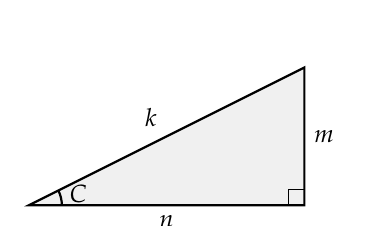
\begin{tikzpicture}[scale=0.7,font=\small]
\draw[thick,FangBlue,fill=FangBlue!6] (0,0)--(5,0)--(5,2.5)--cycle; \draw (4.72,0)--(4.72,0.28)--(5,0.28);
\node[right] at (5,1.25) {$m$}; \node[below] at (2.5,0) {$n$}; \node[above left] at (2.5,1.25) {$k$};
\node[FangRed] at (0.9,0.2) {$C$}; \draw[FangRed,thick] (0.6,0) arc[start angle=0,end angle=26.57,radius=0.6];
\end{tikzpicture}\\[2pt]
\ifkey{\small\color{FangGreen} hyp $r$, opp $p$, adj $q$}\else{\small hyp \underline{\hspace{0.7cm}} opp \underline{\hspace{0.7cm}} adj \underline{\hspace{0.7cm}}}\fi &
\ifkey{\small\color{FangGreen} hyp $z$, opp $y$, adj $x$}\else{\small hyp \underline{\hspace{0.7cm}} opp \underline{\hspace{0.7cm}} adj \underline{\hspace{0.7cm}}}\fi &
\ifkey{\small\color{FangGreen} hyp $k$, opp $m$, adj $n$}\else{\small hyp \underline{\hspace{0.7cm}} opp \underline{\hspace{0.7cm}} adj \underline{\hspace{0.7cm}}}\fi
\end{tabular}
\end{center}

\needspace{7cm}{\large\bfseries\color{FangBlue}B.\ Write the ratios} \easy\ \medium

\textit{Write $\sin A$, $\cos A$ and $\tan A$ as fractions in lowest terms, then as decimals (round to the hundredths).}

\begin{enumerate}[leftmargin=*,label=\textbf{\arabic*.},itemsep=6pt]
\setcounter{enumi}{3}
\np[4.5cm]\item \begin{minipage}[t]{0.3\textwidth}\vspace{0pt}\tri[0.55]{5}{12}{$5$}{$12$}{$13$}{$A$}\end{minipage}\hfill\begin{minipage}[t]{0.62\textwidth}\vspace{0pt}
\work[2.2cm]{opp $5$, adj $12$, hyp $13$. \ $\sin A=\frac{5}{13}\approx0.38$, \ $\cos A=\frac{12}{13}\approx0.92$, \ $\tan A=\frac{5}{12}\approx0.42$.}\end{minipage}
\np[4.5cm]\item \begin{minipage}[t]{0.3\textwidth}\vspace{0pt}\tri[0.32]{15}{8}{$15$}{$8$}{$17$}{$A$}\end{minipage}\hfill\begin{minipage}[t]{0.62\textwidth}\vspace{0pt}
\work[2.2cm]{opp $15$, adj $8$, hyp $17$. \ $\sin A=\frac{15}{17}\approx0.88$, \ $\cos A=\frac{8}{17}\approx0.47$, \ $\tan A=\frac{15}{8}=1.875\approx1.88$. \\ (A tangent \emph{can} be bigger than 1 — when the opposite side is longer than the adjacent.)}\end{minipage}
\np[4.5cm]\item \begin{minipage}[t]{0.3\textwidth}\vspace{0pt}\tri[0.5]{6}{8}{$6$}{$8$}{$10$}{$A$}\end{minipage}\hfill\begin{minipage}[t]{0.62\textwidth}\vspace{0pt}
\work[2.2cm]{$\sin A=\frac{6}{10}=\frac35=0.6$, \ $\cos A=\frac{8}{10}=\frac45=0.8$, \ $\tan A=\frac68=\frac34=0.75$. \\ Same as the $3$-$4$-$5$ triangle — it is a scale drawing (factor $2$), so it has the same angles.}\end{minipage}
\np[3.2cm]\item \medium\ In the triangle of problem 4, now stand at the \textbf{other} sharp angle $B$. Write $\sin B$, $\cos B$ and $\tan B$. What do you notice?
\work[2.2cm]{From $B$: opp $12$, adj $5$, hyp $13$. \ $\sin B=\frac{12}{13}$, \ $\cos B=\frac{5}{13}$, \ $\tan B=\frac{12}{5}$. \\ $\sin B=\cos A$ and $\cos B=\sin A$ — opposite and adjacent swapped. $\tan B$ is the reciprocal of $\tan A$.}
\end{enumerate}

\needspace{6cm}{\large\bfseries\color{FangBlue}C.\ Same angle, same ratio} \medium

\begin{enumerate}[resume,leftmargin=*,label=\textbf{\arabic*.},itemsep=6pt]
\np\item Triangle $P$ has legs $5$ and $12$. Triangle $Q$ has legs $10$ and $24$. Find $\tan$ of the angle across from the short leg in each. Are the two angles equal? Explain.
\work[2.4cm]{$P$: $\tan=\frac{5}{12}$. \ $Q$: $\tan=\frac{10}{24}=\frac{5}{12}$. \ Same ratio, so the angles are equal. $Q$ is a scale drawing of $P$ with scale factor $2$ — scaling changes lengths, not angles.}
\end{enumerate}

\needspace{6cm}{\large\bfseries\color{FangBlue}D.\ Which ratio?} \medium

\textit{Write sin, cos or tan. (Which two sides does the problem use?)}

\begin{enumerate}[resume,leftmargin=*,label=\textbf{\arabic*.},itemsep=4pt]
\item Know the hypotenuse, want the opposite. \work[0.4cm]{sin (SOH)}
\item Know the adjacent, want the opposite. \work[0.4cm]{tan (TOA)}
\item Know the hypotenuse, want the adjacent. \work[0.4cm]{cos (CAH)}
\item Know the opposite, want the hypotenuse. \work[0.4cm]{sin (SOH)}
\end{enumerate}

\needspace{6cm}{\large\bfseries\color{FangBlue}E.\ Find the missing side} \medium\ \hard

\textit{Use the table in Part 4. Draw a picture, label hyp / opp / adj, then solve.}

\begin{enumerate}[resume,leftmargin=*,label=\textbf{\arabic*.},itemsep=6pt]
\np\item \medium\ The hypotenuse is $20$ and one angle is $30^\circ$. Find the side opposite the $30^\circ$ angle.
\work[2.2cm]{$\sin30^\circ=\frac{x}{20}$, \ $0.5=\frac{x}{20}$, \ $x=20\times0.5=10$.}
\np\item \medium\ A ramp is $10$ m long and rises at an angle of $30^\circ$. How high does it go?
\work[2.2cm]{The ramp is the hypotenuse; the height is opposite: $\sin30^\circ=\frac{h}{10}$, \ $h=10\times0.5=5$ m.}
\np\item \medium\ One leg is $8$ and the angle next to it is $45^\circ$. Find the other leg (opposite the $45^\circ$ angle).
\work[2.2cm]{Adjacent $8$, want opposite: $\tan45^\circ=\frac{x}{8}$, \ $1=\frac{x}{8}$, \ $x=8$. \ (A $45^\circ$ right triangle has two equal legs.)}
\np\item \medium\ The hypotenuse is $15$ and one angle is $37^\circ$. Find the side adjacent to the $37^\circ$ angle.
\work[2.2cm]{$\cos37^\circ=\frac{x}{15}$, \ $0.8=\frac{x}{15}$, \ $x=15\times0.8=12$. \ (A $9$-$12$-$15$ triangle — a scaled $3$-$4$-$5$!)}
\np\item \medium\ A tree casts a shadow $12$ m long. From the tip of the shadow, the top of the tree is at an angle of $53^\circ$. How tall is the tree?
\work[2.4cm]{The shadow is adjacent to the $53^\circ$ angle; the tree is opposite. \ $\tan53^\circ=\frac{h}{12}$, \ $h=12\times1.33\approx16$ m.}
\np\item \hard\ The side opposite a $30^\circ$ angle is $7$. Find the hypotenuse.
\work[2.2cm]{$\sin30^\circ=\frac{7}{h}$, \ $0.5=\frac{7}{h}$, \ $h=\frac{7}{0.5}=14$. \ Check: $\frac{7}{14}=0.5$ \checkmark}
\np\item \hard\ A kite string is $50$ m long and makes a $37^\circ$ angle with the ground. How high is the kite? How far away along the ground is it?
\work[2.6cm]{Height (opposite): $50\times\sin37^\circ=50\times0.6=30$ m. \ Ground distance (adjacent): $50\times\cos37^\circ=50\times0.8=40$ m. \ ($30$-$40$-$50$: a scaled $3$-$4$-$5$ triangle.)}
\end{enumerate}

\needspace{6cm}{\large\bfseries\color{FangBlue}F.\ Think about it} \hard

\begin{enumerate}[resume,leftmargin=*,label=\textbf{\arabic*.},itemsep=6pt]
\np\item Why can $\sin A$ never be bigger than $1$?
\work[2cm]{$\sin A=\frac{\text{opposite}}{\text{hypotenuse}}$ and the hypotenuse is the longest side, so the top is smaller than the bottom: the fraction is less than $1$.}
\np\item In a right triangle, $\sin A=\frac35$ and the hypotenuse is $25$. Find the opposite side. Then use $\cos A=\frac45$ to find the adjacent side.
\work[2.2cm]{Opposite $=\frac35\times25=15$. \ Adjacent $=\frac45\times25=20$. \ ($15$-$20$-$25$ is the $3$-$4$-$5$ triangle scaled by $5$.)}
\np\item Why is $\tan45^\circ$ exactly $1$?
\work[2cm]{The angles are $90^\circ$, $45^\circ$, $45^\circ$, so two angles are equal and the two legs are equal. $\tan45^\circ=\frac{\text{opp}}{\text{adj}}=\frac{\text{same}}{\text{same}}=1$.}
\end{enumerate}

\ifkey\else
\vfill
\begin{simple}
\textbf{Remember:} 1) Mark the angle. \ 2) Label hyp, opp, adj from that angle. \ 3) SOH CAH TOA. \ 4) Check: does the hypotenuse come out the longest?
\end{simple}
\fi

\end{document}
"
% =====================================================================
\documentclass[12pt,letterpaper]{article}
\usepackage[margin=0.8in,top=0.85in,bottom=0.8in]{geometry}
\usepackage{mathpazo}
\usepackage[T1]{fontenc}
\usepackage{amsmath,amssymb}
\usepackage{xcolor}
\usepackage{enumitem}
\usepackage{multicol}
\usepackage{booktabs}
\usepackage{needspace}
\usepackage{fancyhdr}
\usepackage[most]{tcolorbox}
\usepackage{pgfplots}
\pgfplotsset{compat=1.17}
\usetikzlibrary{arrows.meta,calc}

\definecolor{FangBlue}{HTML}{1F4E79}
\definecolor{FangTeal}{HTML}{0F7C7C}
\definecolor{FangGold}{HTML}{C9962B}
\definecolor{FangRed}{HTML}{B3261E}
\definecolor{FangGreen}{HTML}{2E8B57}
\definecolor{FangPurple}{HTML}{6A4BD8}
\definecolor{Soft}{HTML}{F4F7FB}
% black-and-white version: pdflatex with \def\isbw{1} before \input
\ifdefined\isbw
\definecolor{FangBlue}{HTML}{000000}\definecolor{FangTeal}{HTML}{000000}\definecolor{FangGold}{HTML}{555555}
\definecolor{FangRed}{HTML}{000000}\definecolor{FangGreen}{HTML}{000000}\definecolor{FangPurple}{HTML}{000000}\definecolor{Soft}{HTML}{FFFFFF}
\fi

\newif\ifkey
\ifdefined\iskey \keytrue \else \keyfalse \fi

\pagestyle{fancy}\fancyhf{}
\renewcommand{\headrulewidth}{0.4pt}
\fancyhead[L]{\small\color{FangBlue}\textbf{FangMath} \,|\, Grade 7 \,·\, First Steps in Trigonometry}
\fancyhead[R]{\small\ifkey\textcolor{FangRed}{\textbf{ANSWER KEY}}\else Name: \underline{\hspace{4.2cm}}\fi}
\fancyfoot[C]{\small\thepage}
\fancyfoot[R]{\scriptsize\color{gray}fangmath.com}
\setlength{\headheight}{14pt}
\setlength{\parindent}{0pt}
\setlength{\parskip}{4pt}

% ---------- boxes ----------
\newtcolorbox{idea}[1][]{colback=Soft,colframe=FangBlue,boxrule=0.8pt,arc=3pt,left=8pt,right=8pt,top=6pt,bottom=6pt,
  fonttitle=\bfseries,coltitle=white,colbacktitle=FangBlue,title={#1}}
\newtcolorbox{example}[1][]{colback=white,colframe=FangTeal,boxrule=0.6pt,arc=3pt,left=8pt,right=8pt,top=5pt,bottom=5pt,
  fonttitle=\bfseries,coltitle=FangTeal,colbacktitle=white,title={#1},attach boxed title to top left={xshift=8pt,yshift=-7pt},boxed title style={boxrule=0pt,colframe=white}, enhanced}
\newtcolorbox{warn}{colback=FangRed!5,colframe=FangRed,boxrule=0.6pt,arc=3pt,left=8pt,right=8pt,top=4pt,bottom=4pt,leftrule=3pt}
\newtcolorbox{simple}{colback=FangGold!10,colframe=FangGold,boxrule=0.6pt,arc=3pt,left=8pt,right=8pt,top=4pt,bottom=4pt,leftrule=3pt}
\newtcolorbox{sol}{colback=FangGreen!6,colframe=FangGreen,boxrule=0.5pt,arc=2pt,left=6pt,right=6pt,top=3pt,bottom=3pt,breakable}

\newcommand{\badge}[2]{\tcbox[on line,colback=#1,colframe=#1,coltext=white,boxrule=0pt,arc=6pt,left=4pt,right=4pt,top=1pt,bottom=1pt,fontupper=\scriptsize\bfseries]{#2}}
\newcommand{\easy}{\badge{FangGreen}{EASY}}
\newcommand{\medium}{\badge{FangTeal}{MEDIUM}}
\newcommand{\hard}{\badge{FangRed}{HARD}}
\newcommand{\work}[2][]{\ifkey\begin{sol}#2\end{sol}\else\vspace*{#1}\fi}
\newcommand{\np}[1][6cm]{\needspace{#1}}
\newcommand{\sect}[2]{\par\needspace{7cm}\medskip{\Large\bfseries\color{FangBlue}\tcbox[on line,colback=FangBlue,colframe=FangBlue,coltext=white,arc=2pt,boxrule=0pt,left=5pt,right=5pt,top=1pt,bottom=1pt]{#1}\ #2}\par\smallskip}

% ---------- right-triangle picture: \rt{scale}{a}{b}{labels...} ----------
% vertices: C = right angle at origin, A = (b,0) [the angle we look from], B = (0,a)
\newcommand{\tri}[7][1]{% #2 #3 = legs (vertical, horizontal); #4 vertical label, #5 horizontal label, #6 hyp label, #7 angle label
\begin{tikzpicture}[scale=#1,font=\small]
\coordinate (C) at (0,0); \coordinate (A) at (#3,0); \coordinate (B) at (0,#2);
\draw[thick,FangBlue,fill=FangBlue!6] (C)--(A)--(B)--cycle;
\draw (0.28,0)--(0.28,0.28)--(0,0.28);
\node[left] at ($(C)!0.5!(B)$) {#4};
\node[below] at ($(C)!0.5!(A)$) {#5};
\node[above right] at ($(A)!0.5!(B)$) {#6};
\node[FangRed] at ($(A)+(-0.75,0.22)$) {#7};
\draw[FangRed,thick] ($(A)+(-0.5,0)$) arc[start angle=180,end angle={180-atan(#2/#3)},radius=0.5];
\end{tikzpicture}}

\begin{document}

% ======================= TITLE =======================
\begin{center}
{\color{FangBlue}\Huge\bfseries First Steps in Trigonometry}\\[3pt]
{\large Sine, Cosine and Tangent — the secret ratios inside every right triangle}
\ifkey\\[3pt]{\color{FangRed}\large\bfseries Answer Key}\fi
\end{center}
\vspace{-2pt}

\begin{idea}[The big idea]
\textbf{Trigonometry} (``triangle measuring'') lets you find a length you \emph{can't} measure — the height of a tree, a building, a kite — from one length and one angle you \emph{can} measure.\par
It works because in a right triangle, \textbf{the angle decides the shape}, and the shape decides the \textbf{ratios} of the sides.
\end{idea}

% ======================= PART 1 =======================
\sect{1}{Name the sides — always from the angle you are looking at}

\begin{minipage}[c]{0.44\textwidth}\centering
\tri[1.05]{3}{4}{\textbf{opposite}}{\textbf{adjacent}}{\textbf{hypotenuse}}{$A$}
\end{minipage}\hfill
\begin{minipage}[c]{0.54\textwidth}
Stand at the angle $A$ (the red arc) and look into the triangle:
\begin{itemize}[leftmargin=*,itemsep=3pt]
\item \textbf{Hypotenuse} — the longest side, \textbf{across from the right angle} $\llcorner$. It never changes.
\item \textbf{Opposite} — the side \textbf{across from} angle $A$. It doesn't touch $A$.
\item \textbf{Adjacent} — the side \textbf{next to} angle $A$ that is \emph{not} the hypotenuse. (``Adjacent'' means ``next to.'')
\end{itemize}
\end{minipage}

\begin{warn}
\textbf{Watch out:} opposite and adjacent \textbf{swap} if you stand at the other sharp angle. Always ask first: ``Which angle am I looking from?''
\end{warn}

% ======================= PART 2 =======================
\sect{2}{Why ratios? A simple case with three triangles}

\begin{minipage}[c]{0.5\textwidth}\centering
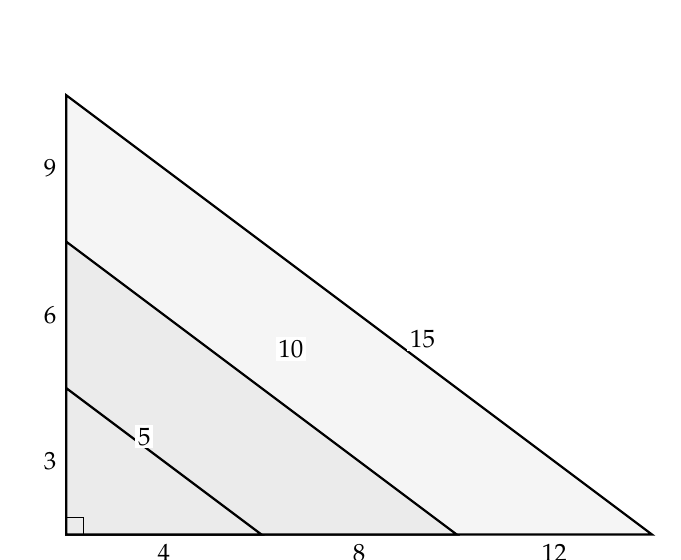
\begin{tikzpicture}[scale=0.62,font=\small]
\draw[thick,FangBlue,fill=FangBlue!4] (0,0)--(12,0)--(0,9)--cycle;
\draw[thick,FangTeal,fill=FangTeal!8] (0,0)--(8,0)--(0,6)--cycle;
\draw[thick,FangRed,fill=FangRed!8] (0,0)--(4,0)--(0,3)--cycle;
\draw (0.35,0)--(0.35,0.35)--(0,0.35);
\node[below,FangRed] at (2,0) {4}; \node[below,FangTeal] at (6,0) {8}; \node[below,FangBlue] at (10,0) {12};
\node[left,FangRed] at (0,1.5) {3}; \node[left,FangTeal] at (0,4.5) {6}; \node[left,FangBlue] at (0,7.5) {9};
\node[FangRed,fill=white,inner sep=1pt] at (1.6,2.0) {5}; \node[FangTeal,fill=white,inner sep=1pt] at (4.6,3.8) {10}; \node[FangBlue,fill=white,inner sep=1pt] at (7.3,4.0) {15};
\node at (-0.6,9.4) {};
\end{tikzpicture}
\end{minipage}\hfill
\begin{minipage}[c]{0.48\textwidth}
These are \textbf{scale drawings} of one triangle (scale factors $1$, $2$, $3$), so they all share the same angles. Look at $\dfrac{\text{opposite}}{\text{hypotenuse}}$ for the bottom-right angle:
\[\frac{3}{5}=0.6 \qquad \frac{6}{10}=0.6 \qquad \frac{9}{15}=0.6\]
\textbf{Same angle $\Rightarrow$ same ratio}, no matter how big the triangle is. These ratios get names: sine, cosine and tangent.
\end{minipage}

% ======================= PART 3 =======================
\sect{3}{The three definitions: SOH CAH TOA}

\begin{idea}[For an acute angle $A$ in a right triangle]
\[
\sin A=\frac{\textbf{O}\text{pposite}}{\textbf{H}\text{ypotenuse}}\qquad\quad
\cos A=\frac{\textbf{A}\text{djacent}}{\textbf{H}\text{ypotenuse}}\qquad\quad
\tan A=\frac{\textbf{O}\text{pposite}}{\textbf{A}\text{djacent}}
\]
\begin{center}\Large\bfseries\color{FangBlue} SOH \quad CAH \quad TOA\end{center}
\centering Memory sentence: \emph{\textbf{S}ome \textbf{O}ld \textbf{H}orses \textbf{C}an \textbf{A}lways \textbf{H}ear \textbf{T}heir \textbf{O}wners \textbf{A}pproach.}
\end{idea}

\begin{example}[Example 1 \;·\; read the ratios]
\begin{minipage}[c]{0.33\textwidth}\centering \tri[0.85]{3}{4}{$3$}{$4$}{$5$}{$A$}\end{minipage}\hfill
\begin{minipage}[c]{0.64\textwidth}
From angle $A$: opposite $=3$, adjacent $=4$, hypotenuse $=5$.
\[\sin A=\frac35=0.6\qquad \cos A=\frac45=0.8\qquad \tan A=\frac34=0.75\]
\textbf{Simple check:} sine and cosine are always \textbf{less than 1}, because the hypotenuse is the longest side.
\end{minipage}
\end{example}

% ======================= PART 4 =======================
\sect{4}{Use a table to find a missing side}

\begin{center}
\renewcommand{\arraystretch}{1.25}
\begin{tabular}{c|ccccc}
\toprule
\textbf{Angle} & $30^\circ$ & $37^\circ$ & $45^\circ$ & $53^\circ$ & $60^\circ$\\ \midrule
$\sin$ & $0.50$ & $0.60$ & $0.71$ & $0.80$ & $0.87$\\
$\cos$ & $0.87$ & $0.80$ & $0.71$ & $0.60$ & $0.50$\\
$\tan$ & $0.58$ & $0.75$ & $1.00$ & $1.33$ & $1.73$\\
\bottomrule
\end{tabular}\\[3pt]
{\small Values are rounded. (A scientific calculator gives them too — make sure it is in \textbf{degree} mode.)}
\end{center}

\begin{idea}[Four steps]
\textbf{1.} Mark the angle you know. \ \textbf{2.} Label the sides: hyp, opp, adj. \ \textbf{3.} Pick the ratio that uses the side you \emph{know} and the side you \emph{want}. \ \textbf{4.} Write the equation and solve it like a proportion.
\end{idea}

\begin{example}[Example 2 \;·\; how high does the ladder reach?]
\begin{minipage}[c]{0.33\textwidth}\centering \tri[0.65]{4.33}{2.5}{$h$\,?}{}{$10$ ft}{$60^\circ$}\end{minipage}\hfill
\begin{minipage}[c]{0.64\textwidth}
A $10$-foot ladder leans on a wall at a $60^\circ$ angle with the ground. \\
Know: hypotenuse $=10$. \ Want: the height, which is \textbf{opposite} the $60^\circ$ angle. \\
Opposite and hypotenuse $\Rightarrow$ \textbf{SOH}, sine:
\[\sin 60^\circ=\frac{h}{10}\ \Rightarrow\ 0.87=\frac{h}{10}\ \Rightarrow\ h=10\times0.87=8.7\ \text{ft}.\]
\end{minipage}
\end{example}

\begin{example}[Example 3 \;·\; the unknown is on the bottom]
The opposite side of a $30^\circ$ angle is $6$. How long is the hypotenuse? \quad
$\sin30^\circ=\dfrac{6}{h}\Rightarrow 0.5=\dfrac{6}{h}\Rightarrow h=\dfrac{6}{0.5}=12.$ \quad \textbf{Check:} $\frac{6}{12}=0.5$ \checkmark
\end{example}

% ======================= PRACTICE =======================
\sect{5}{Practice}

\needspace{6cm}{\large\bfseries\color{FangBlue}A.\ Name the sides} \easy

\textit{For the marked angle, write which side is the hypotenuse, the opposite and the adjacent.}

\begin{center}
\begin{tabular}{ccc}
\textbf{1.} \tri[0.7]{3}{4}{$p$}{$q$}{$r$}{$A$} &
\textbf{2.} 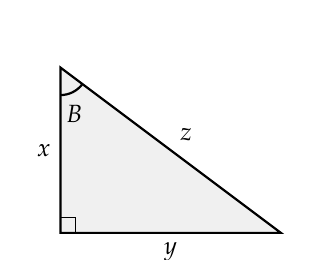
\begin{tikzpicture}[scale=0.7,font=\small]
\draw[thick,FangBlue,fill=FangBlue!6] (0,0)--(4,0)--(0,3)--cycle; \draw (0.28,0)--(0.28,0.28)--(0,0.28);
\node[left] at (0,1.5) {$x$}; \node[below] at (2,0) {$y$}; \node[above right] at (2,1.5) {$z$};
\node[FangRed] at (0.25,2.15) {$B$}; \draw[FangRed,thick] (0,2.5) arc[start angle=270,end angle={270+53.13},radius=0.5];
\end{tikzpicture} &
\textbf{3.} 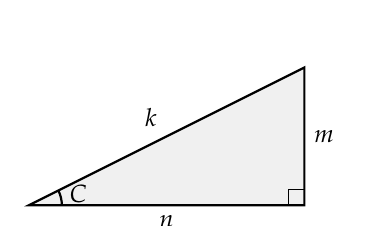
\begin{tikzpicture}[scale=0.7,font=\small]
\draw[thick,FangBlue,fill=FangBlue!6] (0,0)--(5,0)--(5,2.5)--cycle; \draw (4.72,0)--(4.72,0.28)--(5,0.28);
\node[right] at (5,1.25) {$m$}; \node[below] at (2.5,0) {$n$}; \node[above left] at (2.5,1.25) {$k$};
\node[FangRed] at (0.9,0.2) {$C$}; \draw[FangRed,thick] (0.6,0) arc[start angle=0,end angle=26.57,radius=0.6];
\end{tikzpicture}\\[2pt]
\ifkey{\small\color{FangGreen} hyp $r$, opp $p$, adj $q$}\else{\small hyp \underline{\hspace{0.7cm}} opp \underline{\hspace{0.7cm}} adj \underline{\hspace{0.7cm}}}\fi &
\ifkey{\small\color{FangGreen} hyp $z$, opp $y$, adj $x$}\else{\small hyp \underline{\hspace{0.7cm}} opp \underline{\hspace{0.7cm}} adj \underline{\hspace{0.7cm}}}\fi &
\ifkey{\small\color{FangGreen} hyp $k$, opp $m$, adj $n$}\else{\small hyp \underline{\hspace{0.7cm}} opp \underline{\hspace{0.7cm}} adj \underline{\hspace{0.7cm}}}\fi
\end{tabular}
\end{center}

\needspace{7cm}{\large\bfseries\color{FangBlue}B.\ Write the ratios} \easy\ \medium

\textit{Write $\sin A$, $\cos A$ and $\tan A$ as fractions in lowest terms, then as decimals (round to the hundredths).}

\begin{enumerate}[leftmargin=*,label=\textbf{\arabic*.},itemsep=6pt]
\setcounter{enumi}{3}
\np[4.5cm]\item \begin{minipage}[t]{0.3\textwidth}\vspace{0pt}\tri[0.55]{5}{12}{$5$}{$12$}{$13$}{$A$}\end{minipage}\hfill\begin{minipage}[t]{0.62\textwidth}\vspace{0pt}
\work[2.2cm]{opp $5$, adj $12$, hyp $13$. \ $\sin A=\frac{5}{13}\approx0.38$, \ $\cos A=\frac{12}{13}\approx0.92$, \ $\tan A=\frac{5}{12}\approx0.42$.}\end{minipage}
\np[4.5cm]\item \begin{minipage}[t]{0.3\textwidth}\vspace{0pt}\tri[0.32]{15}{8}{$15$}{$8$}{$17$}{$A$}\end{minipage}\hfill\begin{minipage}[t]{0.62\textwidth}\vspace{0pt}
\work[2.2cm]{opp $15$, adj $8$, hyp $17$. \ $\sin A=\frac{15}{17}\approx0.88$, \ $\cos A=\frac{8}{17}\approx0.47$, \ $\tan A=\frac{15}{8}=1.875\approx1.88$. \\ (A tangent \emph{can} be bigger than 1 — when the opposite side is longer than the adjacent.)}\end{minipage}
\np[4.5cm]\item \begin{minipage}[t]{0.3\textwidth}\vspace{0pt}\tri[0.5]{6}{8}{$6$}{$8$}{$10$}{$A$}\end{minipage}\hfill\begin{minipage}[t]{0.62\textwidth}\vspace{0pt}
\work[2.2cm]{$\sin A=\frac{6}{10}=\frac35=0.6$, \ $\cos A=\frac{8}{10}=\frac45=0.8$, \ $\tan A=\frac68=\frac34=0.75$. \\ Same as the $3$-$4$-$5$ triangle — it is a scale drawing (factor $2$), so it has the same angles.}\end{minipage}
\np[3.2cm]\item \medium\ In the triangle of problem 4, now stand at the \textbf{other} sharp angle $B$. Write $\sin B$, $\cos B$ and $\tan B$. What do you notice?
\work[2.2cm]{From $B$: opp $12$, adj $5$, hyp $13$. \ $\sin B=\frac{12}{13}$, \ $\cos B=\frac{5}{13}$, \ $\tan B=\frac{12}{5}$. \\ $\sin B=\cos A$ and $\cos B=\sin A$ — opposite and adjacent swapped. $\tan B$ is the reciprocal of $\tan A$.}
\end{enumerate}

\needspace{6cm}{\large\bfseries\color{FangBlue}C.\ Same angle, same ratio} \medium

\begin{enumerate}[resume,leftmargin=*,label=\textbf{\arabic*.},itemsep=6pt]
\np\item Triangle $P$ has legs $5$ and $12$. Triangle $Q$ has legs $10$ and $24$. Find $\tan$ of the angle across from the short leg in each. Are the two angles equal? Explain.
\work[2.4cm]{$P$: $\tan=\frac{5}{12}$. \ $Q$: $\tan=\frac{10}{24}=\frac{5}{12}$. \ Same ratio, so the angles are equal. $Q$ is a scale drawing of $P$ with scale factor $2$ — scaling changes lengths, not angles.}
\end{enumerate}

\needspace{6cm}{\large\bfseries\color{FangBlue}D.\ Which ratio?} \medium

\textit{Write sin, cos or tan. (Which two sides does the problem use?)}

\begin{enumerate}[resume,leftmargin=*,label=\textbf{\arabic*.},itemsep=4pt]
\item Know the hypotenuse, want the opposite. \work[0.4cm]{sin (SOH)}
\item Know the adjacent, want the opposite. \work[0.4cm]{tan (TOA)}
\item Know the hypotenuse, want the adjacent. \work[0.4cm]{cos (CAH)}
\item Know the opposite, want the hypotenuse. \work[0.4cm]{sin (SOH)}
\end{enumerate}

\needspace{6cm}{\large\bfseries\color{FangBlue}E.\ Find the missing side} \medium\ \hard

\textit{Use the table in Part 4. Draw a picture, label hyp / opp / adj, then solve.}

\begin{enumerate}[resume,leftmargin=*,label=\textbf{\arabic*.},itemsep=6pt]
\np\item \medium\ The hypotenuse is $20$ and one angle is $30^\circ$. Find the side opposite the $30^\circ$ angle.
\work[2.2cm]{$\sin30^\circ=\frac{x}{20}$, \ $0.5=\frac{x}{20}$, \ $x=20\times0.5=10$.}
\np\item \medium\ A ramp is $10$ m long and rises at an angle of $30^\circ$. How high does it go?
\work[2.2cm]{The ramp is the hypotenuse; the height is opposite: $\sin30^\circ=\frac{h}{10}$, \ $h=10\times0.5=5$ m.}
\np\item \medium\ One leg is $8$ and the angle next to it is $45^\circ$. Find the other leg (opposite the $45^\circ$ angle).
\work[2.2cm]{Adjacent $8$, want opposite: $\tan45^\circ=\frac{x}{8}$, \ $1=\frac{x}{8}$, \ $x=8$. \ (A $45^\circ$ right triangle has two equal legs.)}
\np\item \medium\ The hypotenuse is $15$ and one angle is $37^\circ$. Find the side adjacent to the $37^\circ$ angle.
\work[2.2cm]{$\cos37^\circ=\frac{x}{15}$, \ $0.8=\frac{x}{15}$, \ $x=15\times0.8=12$. \ (A $9$-$12$-$15$ triangle — a scaled $3$-$4$-$5$!)}
\np\item \medium\ A tree casts a shadow $12$ m long. From the tip of the shadow, the top of the tree is at an angle of $53^\circ$. How tall is the tree?
\work[2.4cm]{The shadow is adjacent to the $53^\circ$ angle; the tree is opposite. \ $\tan53^\circ=\frac{h}{12}$, \ $h=12\times1.33\approx16$ m.}
\np\item \hard\ The side opposite a $30^\circ$ angle is $7$. Find the hypotenuse.
\work[2.2cm]{$\sin30^\circ=\frac{7}{h}$, \ $0.5=\frac{7}{h}$, \ $h=\frac{7}{0.5}=14$. \ Check: $\frac{7}{14}=0.5$ \checkmark}
\np\item \hard\ A kite string is $50$ m long and makes a $37^\circ$ angle with the ground. How high is the kite? How far away along the ground is it?
\work[2.6cm]{Height (opposite): $50\times\sin37^\circ=50\times0.6=30$ m. \ Ground distance (adjacent): $50\times\cos37^\circ=50\times0.8=40$ m. \ ($30$-$40$-$50$: a scaled $3$-$4$-$5$ triangle.)}
\end{enumerate}

\needspace{6cm}{\large\bfseries\color{FangBlue}F.\ Think about it} \hard

\begin{enumerate}[resume,leftmargin=*,label=\textbf{\arabic*.},itemsep=6pt]
\np\item Why can $\sin A$ never be bigger than $1$?
\work[2cm]{$\sin A=\frac{\text{opposite}}{\text{hypotenuse}}$ and the hypotenuse is the longest side, so the top is smaller than the bottom: the fraction is less than $1$.}
\np\item In a right triangle, $\sin A=\frac35$ and the hypotenuse is $25$. Find the opposite side. Then use $\cos A=\frac45$ to find the adjacent side.
\work[2.2cm]{Opposite $=\frac35\times25=15$. \ Adjacent $=\frac45\times25=20$. \ ($15$-$20$-$25$ is the $3$-$4$-$5$ triangle scaled by $5$.)}
\np\item Why is $\tan45^\circ$ exactly $1$?
\work[2cm]{The angles are $90^\circ$, $45^\circ$, $45^\circ$, so two angles are equal and the two legs are equal. $\tan45^\circ=\frac{\text{opp}}{\text{adj}}=\frac{\text{same}}{\text{same}}=1$.}
\end{enumerate}

\ifkey\else
\vfill
\begin{simple}
\textbf{Remember:} 1) Mark the angle. \ 2) Label hyp, opp, adj from that angle. \ 3) SOH CAH TOA. \ 4) Check: does the hypotenuse come out the longest?
\end{simple}
\fi

\end{document}
"
% =====================================================================
\documentclass[12pt,letterpaper]{article}
\usepackage[margin=0.8in,top=0.85in,bottom=0.8in]{geometry}
\usepackage{mathpazo}
\usepackage[T1]{fontenc}
\usepackage{amsmath,amssymb}
\usepackage{xcolor}
\usepackage{enumitem}
\usepackage{multicol}
\usepackage{booktabs}
\usepackage{needspace}
\usepackage{fancyhdr}
\usepackage[most]{tcolorbox}
\usepackage{pgfplots}
\pgfplotsset{compat=1.17}
\usetikzlibrary{arrows.meta,calc}

\definecolor{FangBlue}{HTML}{1F4E79}
\definecolor{FangTeal}{HTML}{0F7C7C}
\definecolor{FangGold}{HTML}{C9962B}
\definecolor{FangRed}{HTML}{B3261E}
\definecolor{FangGreen}{HTML}{2E8B57}
\definecolor{FangPurple}{HTML}{6A4BD8}
\definecolor{Soft}{HTML}{F4F7FB}
% black-and-white version: pdflatex with \def\isbw{1} before \input
\ifdefined\isbw
\definecolor{FangBlue}{HTML}{000000}\definecolor{FangTeal}{HTML}{000000}\definecolor{FangGold}{HTML}{555555}
\definecolor{FangRed}{HTML}{000000}\definecolor{FangGreen}{HTML}{000000}\definecolor{FangPurple}{HTML}{000000}\definecolor{Soft}{HTML}{FFFFFF}
\fi

\newif\ifkey
\ifdefined\iskey \keytrue \else \keyfalse \fi

\pagestyle{fancy}\fancyhf{}
\renewcommand{\headrulewidth}{0.4pt}
\fancyhead[L]{\small\color{FangBlue}\textbf{FangMath} \,|\, Grade 7 \,·\, First Steps in Trigonometry}
\fancyhead[R]{\small\ifkey\textcolor{FangRed}{\textbf{ANSWER KEY}}\else Name: \underline{\hspace{4.2cm}}\fi}
\fancyfoot[C]{\small\thepage}
\fancyfoot[R]{\scriptsize\color{gray}fangmath.com}
\setlength{\headheight}{14pt}
\setlength{\parindent}{0pt}
\setlength{\parskip}{4pt}

% ---------- boxes ----------
\newtcolorbox{idea}[1][]{colback=Soft,colframe=FangBlue,boxrule=0.8pt,arc=3pt,left=8pt,right=8pt,top=6pt,bottom=6pt,
  fonttitle=\bfseries,coltitle=white,colbacktitle=FangBlue,title={#1}}
\newtcolorbox{example}[1][]{colback=white,colframe=FangTeal,boxrule=0.6pt,arc=3pt,left=8pt,right=8pt,top=5pt,bottom=5pt,
  fonttitle=\bfseries,coltitle=FangTeal,colbacktitle=white,title={#1},attach boxed title to top left={xshift=8pt,yshift=-7pt},boxed title style={boxrule=0pt,colframe=white}, enhanced}
\newtcolorbox{warn}{colback=FangRed!5,colframe=FangRed,boxrule=0.6pt,arc=3pt,left=8pt,right=8pt,top=4pt,bottom=4pt,leftrule=3pt}
\newtcolorbox{simple}{colback=FangGold!10,colframe=FangGold,boxrule=0.6pt,arc=3pt,left=8pt,right=8pt,top=4pt,bottom=4pt,leftrule=3pt}
\newtcolorbox{sol}{colback=FangGreen!6,colframe=FangGreen,boxrule=0.5pt,arc=2pt,left=6pt,right=6pt,top=3pt,bottom=3pt,breakable}

\newcommand{\badge}[2]{\tcbox[on line,colback=#1,colframe=#1,coltext=white,boxrule=0pt,arc=6pt,left=4pt,right=4pt,top=1pt,bottom=1pt,fontupper=\scriptsize\bfseries]{#2}}
\newcommand{\easy}{\badge{FangGreen}{EASY}}
\newcommand{\medium}{\badge{FangTeal}{MEDIUM}}
\newcommand{\hard}{\badge{FangRed}{HARD}}
\newcommand{\work}[2][]{\ifkey\begin{sol}#2\end{sol}\else\vspace*{#1}\fi}
\newcommand{\np}[1][6cm]{\needspace{#1}}
\newcommand{\sect}[2]{\par\needspace{7cm}\medskip{\Large\bfseries\color{FangBlue}\tcbox[on line,colback=FangBlue,colframe=FangBlue,coltext=white,arc=2pt,boxrule=0pt,left=5pt,right=5pt,top=1pt,bottom=1pt]{#1}\ #2}\par\smallskip}

% ---------- right-triangle picture: \rt{scale}{a}{b}{labels...} ----------
% vertices: C = right angle at origin, A = (b,0) [the angle we look from], B = (0,a)
\newcommand{\tri}[7][1]{% #2 #3 = legs (vertical, horizontal); #4 vertical label, #5 horizontal label, #6 hyp label, #7 angle label
\begin{tikzpicture}[scale=#1,font=\small]
\coordinate (C) at (0,0); \coordinate (A) at (#3,0); \coordinate (B) at (0,#2);
\draw[thick,FangBlue,fill=FangBlue!6] (C)--(A)--(B)--cycle;
\draw (0.28,0)--(0.28,0.28)--(0,0.28);
\node[left] at ($(C)!0.5!(B)$) {#4};
\node[below] at ($(C)!0.5!(A)$) {#5};
\node[above right] at ($(A)!0.5!(B)$) {#6};
\node[FangRed] at ($(A)+(-0.75,0.22)$) {#7};
\draw[FangRed,thick] ($(A)+(-0.5,0)$) arc[start angle=180,end angle={180-atan(#2/#3)},radius=0.5];
\end{tikzpicture}}

\begin{document}

% ======================= TITLE =======================
\begin{center}
{\color{FangBlue}\Huge\bfseries First Steps in Trigonometry}\\[3pt]
{\large Sine, Cosine and Tangent — the secret ratios inside every right triangle}
\ifkey\\[3pt]{\color{FangRed}\large\bfseries Answer Key}\fi
\end{center}
\vspace{-2pt}

\begin{idea}[The big idea]
\textbf{Trigonometry} (``triangle measuring'') lets you find a length you \emph{can't} measure — the height of a tree, a building, a kite — from one length and one angle you \emph{can} measure.\par
It works because in a right triangle, \textbf{the angle decides the shape}, and the shape decides the \textbf{ratios} of the sides.
\end{idea}

% ======================= PART 1 =======================
\sect{1}{Name the sides — always from the angle you are looking at}

\begin{minipage}[c]{0.44\textwidth}\centering
\tri[1.05]{3}{4}{\textbf{opposite}}{\textbf{adjacent}}{\textbf{hypotenuse}}{$A$}
\end{minipage}\hfill
\begin{minipage}[c]{0.54\textwidth}
Stand at the angle $A$ (the red arc) and look into the triangle:
\begin{itemize}[leftmargin=*,itemsep=3pt]
\item \textbf{Hypotenuse} — the longest side, \textbf{across from the right angle} $\llcorner$. It never changes.
\item \textbf{Opposite} — the side \textbf{across from} angle $A$. It doesn't touch $A$.
\item \textbf{Adjacent} — the side \textbf{next to} angle $A$ that is \emph{not} the hypotenuse. (``Adjacent'' means ``next to.'')
\end{itemize}
\end{minipage}

\begin{warn}
\textbf{Watch out:} opposite and adjacent \textbf{swap} if you stand at the other sharp angle. Always ask first: ``Which angle am I looking from?''
\end{warn}

% ======================= PART 2 =======================
\sect{2}{Why ratios? A simple case with three triangles}

\begin{minipage}[c]{0.5\textwidth}\centering
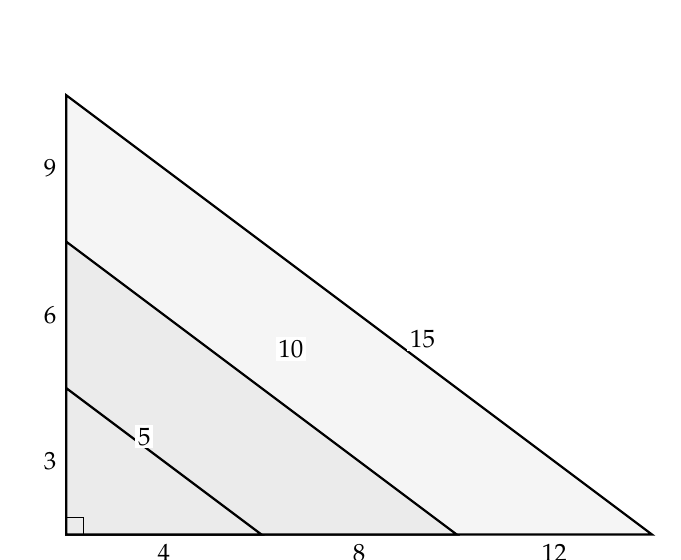
\begin{tikzpicture}[scale=0.62,font=\small]
\draw[thick,FangBlue,fill=FangBlue!4] (0,0)--(12,0)--(0,9)--cycle;
\draw[thick,FangTeal,fill=FangTeal!8] (0,0)--(8,0)--(0,6)--cycle;
\draw[thick,FangRed,fill=FangRed!8] (0,0)--(4,0)--(0,3)--cycle;
\draw (0.35,0)--(0.35,0.35)--(0,0.35);
\node[below,FangRed] at (2,0) {4}; \node[below,FangTeal] at (6,0) {8}; \node[below,FangBlue] at (10,0) {12};
\node[left,FangRed] at (0,1.5) {3}; \node[left,FangTeal] at (0,4.5) {6}; \node[left,FangBlue] at (0,7.5) {9};
\node[FangRed,fill=white,inner sep=1pt] at (1.6,2.0) {5}; \node[FangTeal,fill=white,inner sep=1pt] at (4.6,3.8) {10}; \node[FangBlue,fill=white,inner sep=1pt] at (7.3,4.0) {15};
\node at (-0.6,9.4) {};
\end{tikzpicture}
\end{minipage}\hfill
\begin{minipage}[c]{0.48\textwidth}
These are \textbf{scale drawings} of one triangle (scale factors $1$, $2$, $3$), so they all share the same angles. Look at $\dfrac{\text{opposite}}{\text{hypotenuse}}$ for the bottom-right angle:
\[\frac{3}{5}=0.6 \qquad \frac{6}{10}=0.6 \qquad \frac{9}{15}=0.6\]
\textbf{Same angle $\Rightarrow$ same ratio}, no matter how big the triangle is. These ratios get names: sine, cosine and tangent.
\end{minipage}

% ======================= PART 3 =======================
\sect{3}{The three definitions: SOH CAH TOA}

\begin{idea}[For an acute angle $A$ in a right triangle]
\[
\sin A=\frac{\textbf{O}\text{pposite}}{\textbf{H}\text{ypotenuse}}\qquad\quad
\cos A=\frac{\textbf{A}\text{djacent}}{\textbf{H}\text{ypotenuse}}\qquad\quad
\tan A=\frac{\textbf{O}\text{pposite}}{\textbf{A}\text{djacent}}
\]
\begin{center}\Large\bfseries\color{FangBlue} SOH \quad CAH \quad TOA\end{center}
\centering Memory sentence: \emph{\textbf{S}ome \textbf{O}ld \textbf{H}orses \textbf{C}an \textbf{A}lways \textbf{H}ear \textbf{T}heir \textbf{O}wners \textbf{A}pproach.}
\end{idea}

\begin{example}[Example 1 \;·\; read the ratios]
\begin{minipage}[c]{0.33\textwidth}\centering \tri[0.85]{3}{4}{$3$}{$4$}{$5$}{$A$}\end{minipage}\hfill
\begin{minipage}[c]{0.64\textwidth}
From angle $A$: opposite $=3$, adjacent $=4$, hypotenuse $=5$.
\[\sin A=\frac35=0.6\qquad \cos A=\frac45=0.8\qquad \tan A=\frac34=0.75\]
\textbf{Simple check:} sine and cosine are always \textbf{less than 1}, because the hypotenuse is the longest side.
\end{minipage}
\end{example}

% ======================= PART 4 =======================
\sect{4}{Use a table to find a missing side}

\begin{center}
\renewcommand{\arraystretch}{1.25}
\begin{tabular}{c|ccccc}
\toprule
\textbf{Angle} & $30^\circ$ & $37^\circ$ & $45^\circ$ & $53^\circ$ & $60^\circ$\\ \midrule
$\sin$ & $0.50$ & $0.60$ & $0.71$ & $0.80$ & $0.87$\\
$\cos$ & $0.87$ & $0.80$ & $0.71$ & $0.60$ & $0.50$\\
$\tan$ & $0.58$ & $0.75$ & $1.00$ & $1.33$ & $1.73$\\
\bottomrule
\end{tabular}\\[3pt]
{\small Values are rounded. (A scientific calculator gives them too — make sure it is in \textbf{degree} mode.)}
\end{center}

\begin{idea}[Four steps]
\textbf{1.} Mark the angle you know. \ \textbf{2.} Label the sides: hyp, opp, adj. \ \textbf{3.} Pick the ratio that uses the side you \emph{know} and the side you \emph{want}. \ \textbf{4.} Write the equation and solve it like a proportion.
\end{idea}

\begin{example}[Example 2 \;·\; how high does the ladder reach?]
\begin{minipage}[c]{0.33\textwidth}\centering \tri[0.65]{4.33}{2.5}{$h$\,?}{}{$10$ ft}{$60^\circ$}\end{minipage}\hfill
\begin{minipage}[c]{0.64\textwidth}
A $10$-foot ladder leans on a wall at a $60^\circ$ angle with the ground. \\
Know: hypotenuse $=10$. \ Want: the height, which is \textbf{opposite} the $60^\circ$ angle. \\
Opposite and hypotenuse $\Rightarrow$ \textbf{SOH}, sine:
\[\sin 60^\circ=\frac{h}{10}\ \Rightarrow\ 0.87=\frac{h}{10}\ \Rightarrow\ h=10\times0.87=8.7\ \text{ft}.\]
\end{minipage}
\end{example}

\begin{example}[Example 3 \;·\; the unknown is on the bottom]
The opposite side of a $30^\circ$ angle is $6$. How long is the hypotenuse? \quad
$\sin30^\circ=\dfrac{6}{h}\Rightarrow 0.5=\dfrac{6}{h}\Rightarrow h=\dfrac{6}{0.5}=12.$ \quad \textbf{Check:} $\frac{6}{12}=0.5$ \checkmark
\end{example}

% ======================= PRACTICE =======================
\sect{5}{Practice}

\needspace{6cm}{\large\bfseries\color{FangBlue}A.\ Name the sides} \easy

\textit{For the marked angle, write which side is the hypotenuse, the opposite and the adjacent.}

\begin{center}
\begin{tabular}{ccc}
\textbf{1.} \tri[0.7]{3}{4}{$p$}{$q$}{$r$}{$A$} &
\textbf{2.} 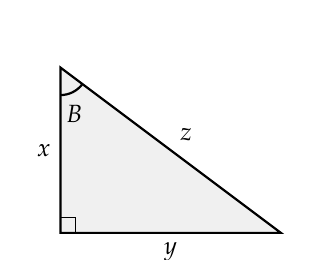
\begin{tikzpicture}[scale=0.7,font=\small]
\draw[thick,FangBlue,fill=FangBlue!6] (0,0)--(4,0)--(0,3)--cycle; \draw (0.28,0)--(0.28,0.28)--(0,0.28);
\node[left] at (0,1.5) {$x$}; \node[below] at (2,0) {$y$}; \node[above right] at (2,1.5) {$z$};
\node[FangRed] at (0.25,2.15) {$B$}; \draw[FangRed,thick] (0,2.5) arc[start angle=270,end angle={270+53.13},radius=0.5];
\end{tikzpicture} &
\textbf{3.} 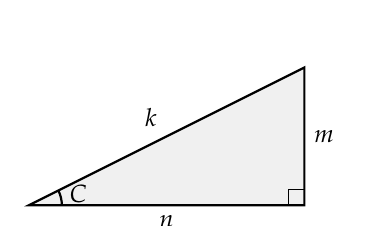
\begin{tikzpicture}[scale=0.7,font=\small]
\draw[thick,FangBlue,fill=FangBlue!6] (0,0)--(5,0)--(5,2.5)--cycle; \draw (4.72,0)--(4.72,0.28)--(5,0.28);
\node[right] at (5,1.25) {$m$}; \node[below] at (2.5,0) {$n$}; \node[above left] at (2.5,1.25) {$k$};
\node[FangRed] at (0.9,0.2) {$C$}; \draw[FangRed,thick] (0.6,0) arc[start angle=0,end angle=26.57,radius=0.6];
\end{tikzpicture}\\[2pt]
\ifkey{\small\color{FangGreen} hyp $r$, opp $p$, adj $q$}\else{\small hyp \underline{\hspace{0.7cm}} opp \underline{\hspace{0.7cm}} adj \underline{\hspace{0.7cm}}}\fi &
\ifkey{\small\color{FangGreen} hyp $z$, opp $y$, adj $x$}\else{\small hyp \underline{\hspace{0.7cm}} opp \underline{\hspace{0.7cm}} adj \underline{\hspace{0.7cm}}}\fi &
\ifkey{\small\color{FangGreen} hyp $k$, opp $m$, adj $n$}\else{\small hyp \underline{\hspace{0.7cm}} opp \underline{\hspace{0.7cm}} adj \underline{\hspace{0.7cm}}}\fi
\end{tabular}
\end{center}

\needspace{7cm}{\large\bfseries\color{FangBlue}B.\ Write the ratios} \easy\ \medium

\textit{Write $\sin A$, $\cos A$ and $\tan A$ as fractions in lowest terms, then as decimals (round to the hundredths).}

\begin{enumerate}[leftmargin=*,label=\textbf{\arabic*.},itemsep=6pt]
\setcounter{enumi}{3}
\np[4.5cm]\item \begin{minipage}[t]{0.3\textwidth}\vspace{0pt}\tri[0.55]{5}{12}{$5$}{$12$}{$13$}{$A$}\end{minipage}\hfill\begin{minipage}[t]{0.62\textwidth}\vspace{0pt}
\work[2.2cm]{opp $5$, adj $12$, hyp $13$. \ $\sin A=\frac{5}{13}\approx0.38$, \ $\cos A=\frac{12}{13}\approx0.92$, \ $\tan A=\frac{5}{12}\approx0.42$.}\end{minipage}
\np[4.5cm]\item \begin{minipage}[t]{0.3\textwidth}\vspace{0pt}\tri[0.32]{15}{8}{$15$}{$8$}{$17$}{$A$}\end{minipage}\hfill\begin{minipage}[t]{0.62\textwidth}\vspace{0pt}
\work[2.2cm]{opp $15$, adj $8$, hyp $17$. \ $\sin A=\frac{15}{17}\approx0.88$, \ $\cos A=\frac{8}{17}\approx0.47$, \ $\tan A=\frac{15}{8}=1.875\approx1.88$. \\ (A tangent \emph{can} be bigger than 1 — when the opposite side is longer than the adjacent.)}\end{minipage}
\np[4.5cm]\item \begin{minipage}[t]{0.3\textwidth}\vspace{0pt}\tri[0.5]{6}{8}{$6$}{$8$}{$10$}{$A$}\end{minipage}\hfill\begin{minipage}[t]{0.62\textwidth}\vspace{0pt}
\work[2.2cm]{$\sin A=\frac{6}{10}=\frac35=0.6$, \ $\cos A=\frac{8}{10}=\frac45=0.8$, \ $\tan A=\frac68=\frac34=0.75$. \\ Same as the $3$-$4$-$5$ triangle — it is a scale drawing (factor $2$), so it has the same angles.}\end{minipage}
\np[3.2cm]\item \medium\ In the triangle of problem 4, now stand at the \textbf{other} sharp angle $B$. Write $\sin B$, $\cos B$ and $\tan B$. What do you notice?
\work[2.2cm]{From $B$: opp $12$, adj $5$, hyp $13$. \ $\sin B=\frac{12}{13}$, \ $\cos B=\frac{5}{13}$, \ $\tan B=\frac{12}{5}$. \\ $\sin B=\cos A$ and $\cos B=\sin A$ — opposite and adjacent swapped. $\tan B$ is the reciprocal of $\tan A$.}
\end{enumerate}

\needspace{6cm}{\large\bfseries\color{FangBlue}C.\ Same angle, same ratio} \medium

\begin{enumerate}[resume,leftmargin=*,label=\textbf{\arabic*.},itemsep=6pt]
\np\item Triangle $P$ has legs $5$ and $12$. Triangle $Q$ has legs $10$ and $24$. Find $\tan$ of the angle across from the short leg in each. Are the two angles equal? Explain.
\work[2.4cm]{$P$: $\tan=\frac{5}{12}$. \ $Q$: $\tan=\frac{10}{24}=\frac{5}{12}$. \ Same ratio, so the angles are equal. $Q$ is a scale drawing of $P$ with scale factor $2$ — scaling changes lengths, not angles.}
\end{enumerate}

\needspace{6cm}{\large\bfseries\color{FangBlue}D.\ Which ratio?} \medium

\textit{Write sin, cos or tan. (Which two sides does the problem use?)}

\begin{enumerate}[resume,leftmargin=*,label=\textbf{\arabic*.},itemsep=4pt]
\item Know the hypotenuse, want the opposite. \work[0.4cm]{sin (SOH)}
\item Know the adjacent, want the opposite. \work[0.4cm]{tan (TOA)}
\item Know the hypotenuse, want the adjacent. \work[0.4cm]{cos (CAH)}
\item Know the opposite, want the hypotenuse. \work[0.4cm]{sin (SOH)}
\end{enumerate}

\needspace{6cm}{\large\bfseries\color{FangBlue}E.\ Find the missing side} \medium\ \hard

\textit{Use the table in Part 4. Draw a picture, label hyp / opp / adj, then solve.}

\begin{enumerate}[resume,leftmargin=*,label=\textbf{\arabic*.},itemsep=6pt]
\np\item \medium\ The hypotenuse is $20$ and one angle is $30^\circ$. Find the side opposite the $30^\circ$ angle.
\work[2.2cm]{$\sin30^\circ=\frac{x}{20}$, \ $0.5=\frac{x}{20}$, \ $x=20\times0.5=10$.}
\np\item \medium\ A ramp is $10$ m long and rises at an angle of $30^\circ$. How high does it go?
\work[2.2cm]{The ramp is the hypotenuse; the height is opposite: $\sin30^\circ=\frac{h}{10}$, \ $h=10\times0.5=5$ m.}
\np\item \medium\ One leg is $8$ and the angle next to it is $45^\circ$. Find the other leg (opposite the $45^\circ$ angle).
\work[2.2cm]{Adjacent $8$, want opposite: $\tan45^\circ=\frac{x}{8}$, \ $1=\frac{x}{8}$, \ $x=8$. \ (A $45^\circ$ right triangle has two equal legs.)}
\np\item \medium\ The hypotenuse is $15$ and one angle is $37^\circ$. Find the side adjacent to the $37^\circ$ angle.
\work[2.2cm]{$\cos37^\circ=\frac{x}{15}$, \ $0.8=\frac{x}{15}$, \ $x=15\times0.8=12$. \ (A $9$-$12$-$15$ triangle — a scaled $3$-$4$-$5$!)}
\np\item \medium\ A tree casts a shadow $12$ m long. From the tip of the shadow, the top of the tree is at an angle of $53^\circ$. How tall is the tree?
\work[2.4cm]{The shadow is adjacent to the $53^\circ$ angle; the tree is opposite. \ $\tan53^\circ=\frac{h}{12}$, \ $h=12\times1.33\approx16$ m.}
\np\item \hard\ The side opposite a $30^\circ$ angle is $7$. Find the hypotenuse.
\work[2.2cm]{$\sin30^\circ=\frac{7}{h}$, \ $0.5=\frac{7}{h}$, \ $h=\frac{7}{0.5}=14$. \ Check: $\frac{7}{14}=0.5$ \checkmark}
\np\item \hard\ A kite string is $50$ m long and makes a $37^\circ$ angle with the ground. How high is the kite? How far away along the ground is it?
\work[2.6cm]{Height (opposite): $50\times\sin37^\circ=50\times0.6=30$ m. \ Ground distance (adjacent): $50\times\cos37^\circ=50\times0.8=40$ m. \ ($30$-$40$-$50$: a scaled $3$-$4$-$5$ triangle.)}
\end{enumerate}

\needspace{6cm}{\large\bfseries\color{FangBlue}F.\ Think about it} \hard

\begin{enumerate}[resume,leftmargin=*,label=\textbf{\arabic*.},itemsep=6pt]
\np\item Why can $\sin A$ never be bigger than $1$?
\work[2cm]{$\sin A=\frac{\text{opposite}}{\text{hypotenuse}}$ and the hypotenuse is the longest side, so the top is smaller than the bottom: the fraction is less than $1$.}
\np\item In a right triangle, $\sin A=\frac35$ and the hypotenuse is $25$. Find the opposite side. Then use $\cos A=\frac45$ to find the adjacent side.
\work[2.2cm]{Opposite $=\frac35\times25=15$. \ Adjacent $=\frac45\times25=20$. \ ($15$-$20$-$25$ is the $3$-$4$-$5$ triangle scaled by $5$.)}
\np\item Why is $\tan45^\circ$ exactly $1$?
\work[2cm]{The angles are $90^\circ$, $45^\circ$, $45^\circ$, so two angles are equal and the two legs are equal. $\tan45^\circ=\frac{\text{opp}}{\text{adj}}=\frac{\text{same}}{\text{same}}=1$.}
\end{enumerate}

\ifkey\else
\vfill
\begin{simple}
\textbf{Remember:} 1) Mark the angle. \ 2) Label hyp, opp, adj from that angle. \ 3) SOH CAH TOA. \ 4) Check: does the hypotenuse come out the longest?
\end{simple}
\fi

\end{document}
